\documentclass[11pt]{article}

\usepackage[margin=1in]{geometry}
\usepackage{amsmath, amssymb}
\usepackage{authblk}
\usepackage{booktabs}
\usepackage{tabularx}
\usepackage{longtable}
\usepackage{pdflscape}
\usepackage{graphicx}
\usepackage{caption}
\usepackage{subcaption}
\usepackage{algorithm}
\usepackage{algpseudocode}
\usepackage[hidelinks]{hyperref}
\usepackage[style=apa, version=7]{biblatex}
\addbibresource{bib.bib}

\newcommand{\psuccess}{P(\text{success})}
\newcommand{\law}{\mathcal{L}}
\newcommand{\wtsq}{W_2^2}

\title{Toward Fragility-Guided Elicitation Budget Allocation for \\ AI-Cyber Risk Modeling with Bayesian Networks}

\author[1]{James Sykes}
\author[2]{Jakub Kry\'{s}}
\author[2]{Matthew Smith}

\affil[1]{Department of Statistics, University of Warwick}
\affil[2]{SaferAI}
\date{}

\begin{document}

\maketitle

\begin{abstract}
SaferAI’s quantitative AI-cyber risk models are parameterized with probability distributions elicited from experts, and this expert elicitation process often proves to be an expensive bottleneck. This report investigates whether elicitation effort can be allocated more efficiently by prioritizing inputs that appear to have the greatest effect on the output probability distribution. In order to investigate this, we perform a retrospective budget-recovery experiment on SaferAI’s OC3 Denial-of-Service risk model, restricted to the SOTA capability condition and the $P(\text{success})$ submodel. The experiment compares a uniform baseline with several fragility-guided allocation heuristics. The results support further investigation of non-uniform elicitation allocation, but they do not clearly support the use of this particular fragility-guided heuristic.
\end{abstract}

\tableofcontents
\newpage

\section{Introduction}

SaferAI's current approach to quantitative AI-cyber risk modeling relies on eliciting probability distributions from experts in order to parameterize a Bayesian network-based risk model (\cite{barrett2025toward}). This is an inherently expensive process to undertake, both in terms of the time required and the expense, a problem commonly referred to as ``the elicitation burden'' (\cite{barons2022balancing}). While LLM-based expert elicitation is increasingly being regarded as a viable way of eliciting the required information in a cheaper manner (\cite{halawi2024approaching}), the cost of doing this remains far from negligible. As a result, there is a strong motivation for us to develop methods to improve the efficiency of the expert elicitation process.

There is little existing work on this problem, partly because AI-cyber risk modeling is still a nascent field. We take inspiration from the experimental design literature, particularly that on active learning (\cite{settles2009active}). Active learning deals with the intelligent collection of data to train a machine learning model, via the use of an acquisition function, which assigns a score at each ``sampling opportunity'' to every point in the input space as to how desirable it would be to sample there. While the machinery we use does not fall under the remit of active learning, our approach is similar: we score the desirability of potential information we could elicit, and then use this to decide which nodes of the Bayesian network to elicit information for at each stage of the process.

Motivated by the assumption that the output distribution is more sensitive to some parts of the risk model than others, we investigate the use of a simple ``leave-one-out'' (LOO) heuristic as the basis for an acquisition function to inform the allocation of our elicitation budget. We experiment with several different policies for budget allocation, each relying on the same LOO heuristic, and then compare these to uniform sampling. Specifically, we examine whether our heuristic can improve the recovery of a full-data reference output distribution when we are given a limited elicitation budget. We then discuss limitations of our approach and potential ways to develop this work from here.

\section{Methods}
\subsection{Experiment scope}
The scope of our experiments is intentionally narrow, utilizing a submodel of SaferAI's OC3 Denial of Service risk model (\cite{barrett2025toward}). Specifically, we retain all the nodes\footnote{In what follows, we refer to the random variables of a Bayesian network as nodes.} in the original model with the exception of \texttt{Rate of Successful Attempt}, \texttt{Number of Successful Attacks}, \texttt{Total Risk}, and the parents of these nodes, \texttt{Number of Attempts per Actor}, \texttt{Number of Actors}, and \texttt{Damage per Attack}. Consequently, our experiments do not model the full total-risk equation. That is, rather than consider our output to be the probability distribution of \texttt{Total Risk}, we consider it to be the probability distribution of \texttt{Successful Attack Rate}. Hereafter, rather than use this full name, we refer to \texttt{Successful Attack Rate}, when in the context of it being the output of the risk model under consideration, as $\psuccess$. 

More formally, we write that our output is
\begin{equation} \label{output function}
    T(M)=\law\left(P_M(\mathrm{success})\right),
\end{equation}
where we use $T$ to denote a function that maps the current 9-tuple $M$ of nodewise elicitation mixtures to the output distribution under consideration. Here, $M = (M_1,\dots,M_9)$, where $M_j$ is the mixture distribution for node $j$. Also, note that $\law(X)$ denotes the law, or probability distribution, of $X$.

An additional simplification we make is to fix the inputs of our risk model to the state-of-the-art (SOTA) levels\footnote{Here, the SOTA level for the CyBench benchmark is \texttt{Labyrinth Linguist} and for BountyBench it is \texttt{Paddle}.}. This is sufficient for our objectives, since we consider our sample space to be node--expert pairs --- we want the capability inputs to the risk model to be fixed. This would remain the case even if we considered many (or even all) of the possible combinations of inputs to the risk model.

\subsection{Fitting elicitation distributions}

The dataset used for this experiment contains 1800 rows\footnote{Note that two rows are not valid due to API timeouts, and have therefore been excluded from the subsequent experiments.}:
\[
40 \text{ repeats} \times 5 \text{ LLM forecaster models} \times 9 \text{ nodes} \times 1 \text{ capability level}.
\]
Rows include elicited probability quartiles $\texttt{percentile\_25th}$, $\texttt{percentile\_50th}$, and $\texttt{percentile\_75th}$. There is also an $\texttt{estimate}$ column, in accordance with SaferAI's current elicitation protocol, but this is not used for fitting probability distributions to the information provided by the experts\footnote{For simplicity, we refer to both humans and LLMs who provide probability distributions to parametrize risk models as ``experts''.}.

Each elicitation row gives three quartiles $(q_{0.25},q_{0.50},q_{0.75})$ for one node probability. The implementation fits one Beta distribution on $[0,1]$ to each row by quantile matching:
\[
(\hat{\alpha},\hat{\beta})
=
\arg\min_{\alpha,\beta>0}
\sum_{\tau \in \{0.25,0.50,0.75\}}
\left[
Q_{\mathrm{Beta}}(\tau;\alpha,\beta)-q_{\tau}
\right]^2.
\]
Note that, letting $X \sim \mu$, we have \[Q_{\mu}(\tau) = \inf\{x: \mathbb{P}(X\leq x) \geq \tau\}.\]
Optimization is performed in log-parameter space so that $\alpha,\beta>0$.

\subsection{OC3 DoS \texorpdfstring{$P(\mathrm{success})$}{P(success)} submodel}

The OC3 DoS $\psuccess$ submodel has nine nodes (each is a MITRE ATT\&CK technique) for which probability distributions were directly elicited:
\[
\begin{array}{ll}
p_{\mathrm{active}} & \text{T1595 -- Reconnaissance: Active Scanning},\\
p_{\mathrm{gather}} & \text{T1590 -- Reconnaissance: Gather Victim Network Information},\\
p_{\mathrm{acquire}} & \text{T1583.005 -- Resource Development: Acquire Botnet},\\
p_{\mathrm{build}} & \text{T1584.005 -- Resource Development: Build/Compromise Botnet},\\
p_{\mathrm{masq}} & \text{T1036 -- Defense Evasion: Masquerading},\\
p_{\mathrm{port}} & \text{T1571 -- Defense Evasion: Non-Standard Port},\\
p_{\mathrm{c2}} & \text{TA0011 -- Command-and-Control},\\
p_{\mathrm{direct}} & \text{T1498.001 -- Impact: Direct Network Flood},\\
p_{\mathrm{refl}} & \text{T1498.002 -- Impact: Reflection/Amplification Attack}.
\end{array}
\]

These technique-level probabilities are aggregated into the following tactic-level quantities:
\[
\begin{array}{ll}
p_{\mathrm{rec}} & \text{TA0043 -- Reconnaissance},\\
p_{\mathrm{res}} & \text{TA0042 -- Resource Development},\\
p_{\mathrm{def}} & \text{TA0030 -- Defense Evasion},\\
p_{\mathrm{imp}} & \text{TA0040 -- Impact}
\end{array}
\]

Each is either an AND or an OR gate:
\begin{align*}
p_{\mathrm{rec}} &= p_{\mathrm{active}} + p_{\mathrm{gather}} - p_{\mathrm{active}}p_{\mathrm{gather}}, \tag*{(OR gate)}\\
p_{\mathrm{res}} &= p_{\mathrm{build}} + p_{\mathrm{acquire}} - p_{\mathrm{build}}p_{\mathrm{acquire}}, \tag*{(OR gate)}\\
p_{\mathrm{def}} &= p_{\mathrm{port}}p_{\mathrm{masq}}, \tag*{(AND gate)}\\
p_{\mathrm{imp}} &= p_{\mathrm{direct}} + p_{\mathrm{refl}} - p_{\mathrm{direct}}p_{\mathrm{refl}} \tag*{(OR gate)}.
\end{align*}
The final success probability is
\[
\psuccess
=
p_{\mathrm{rec}}p_{\mathrm{res}}p_{\mathrm{def}}p_{\mathrm{c2}}p_{\mathrm{imp}}.
\]

\subsection{Exchangeable nodewise mixtures}

For node $j$, let $S_j$ be the set of currently revealed draws. The current node mixture distribution is
\[
M_j(S_j)=\frac{1}{|S_j|}\sum_{d\in S_j}D_{j,d},
\]
where $D_{j,d}$ is the fitted Beta distribution for draw $d$ at node $j$. To sample from $M_j$, the implementation chooses a revealed fitted row uniformly and then samples from its Beta distribution. Node samples are drawn independently across the nine nodes before propagation through the risk model.

\subsection{Full-data reference distribution}

The full-data reference uses all rows for each node:
\[
M_j^{\mathrm{full}}
=
\frac{1}{|S_j^{\mathrm{full}}|}
\sum_{d\in S_j^{\mathrm{full}}}D_{j,d}.
\]
This provides us with the full-data model $M^{\mathrm{full}} = (M^{\mathrm{full}}_1,\dots,M^{\mathrm{full}}_9)$.
Then, the reference output distribution, as implied by (\ref{output function}), is
\[
T(M^{\mathrm{full}})=\law\left(P_{M^{\mathrm{full}}}(\mathrm{success})\right).
\]

\subsection{Budgeted reveal protocol}

For each ``reveal seed'', the experiment has a specified reveal order for each node. For each of these, repeats are shuffled for each of the five LLMs to obtain a random order for that seed and model. All policies begin with the same initial seed allocation: five rows for each node, one from each LLM, for a total initial budget of 45 SOTA elicitation rows. After this initial seed allocation, a policy selects the next node. When it selects node $j$, it receives the next unused fitted row for $j$ from the seed-specific reveal order. This ensures that, under a given reveal seed, policies differ only in which node they choose to reveal next, not in the hidden ordering of rows within each node.

\begin{algorithm}[htbp]
\caption{Retrospective budget-recovery experiment for one reveal seed and policy}
\label{alg:budget-recovery}
\begin{algorithmic}[1]
\Require Fitted elicitation-row pools $\{D_{j,d}\}$ for nodes $j=1,\ldots,9$; hidden reveal orders $\{\pi_j\}_{j=1}^9$; allocation policy $\mathcal{A}$; budget grid $\mathcal{B}$; full-data reference distribution $T(M^{\mathrm{full}})$
\State Initialize each revealed set $S_j$ with one row from each LLM forecaster model
\State Set total revealed budget $b \gets \sum_{j=1}^9 |S_j| = 45$
\State Estimate $T(M(S_1,\ldots,S_9))$ by Monte Carlo sampling and record error to $T(M^{\mathrm{full}})$ at budget $b$
\While{$b < \max(\mathcal{B})$}
    \If{fragility scores are required by $\mathcal{A}$ and due for recomputation}
        \State Estimate current LOO fragility scores $\{F_j^{\mathrm{LOO}}\}_{j=1}^9$
    \EndIf
    \State Let $\mathcal{J}_{\mathrm{eligible}} \gets \{j : \pi_j \text{ has at least one unrevealed row}\}$
    \State Choose next node $j^\star \sim \mathcal{A}\!\left(\{S_j\}_{j=1}^9,\{F_j^{\mathrm{LOO}}\}_{j=1}^9,\mathcal{J}_{\mathrm{eligible}}\right)$
    \State Reveal the next unused row for node $j^\star$ according to $\pi_{j^\star}$ and add it to $S_{j^\star}$
    \State Set $b \gets b+1$
    \If{$b \in \mathcal{B}$}
        \State Estimate $T(M(S_1,\ldots,S_9))$ by Monte Carlo sampling
        \State Record squared Wasserstein-2 error to $T(M^{\mathrm{full}})$
    \EndIf
\EndWhile
\end{algorithmic}
\end{algorithm}

\subsection{LOO output fragility}

Given revealed draw sets $S_1,\ldots,S_9$, let $M$ be the current exchangeable nodewise mixture model. For a draw $d\in S_j$, define
\[
M_j^{(-d)}
=
\frac{1}{|S_j|-1}
\sum_{d'\in S_j,\,d'\neq d}D_{j,d'}.
\]
Let $M^{(j,-d)}$ be the model equal to $M$ except that node $j$'s mixture is replaced by $M_j^{(-d)}$. That is, \[M^{(j,-d)} = (M_1,\dots,M_{j-1},M_j^{(-d)},M_{j+1},\dots,M_9).\]
The LOO fragility score is then an average of distances between the output distributions when using the LOO models and when using the current model:
\[
F_j^{\mathrm{LOO}}
=
\frac{1}{|S_j|}
\sum_{d\in S_j}
\wtsq\left(T(M^{(j,-d)}),T(M)\right),
\]
where $W_2$ is the Wasserstein-2 distance (\cite{villani2009optimal}).

\subsection{Allocation policies}

The implemented policy families are:
\begin{enumerate}
    \item \textbf{Uniform allocation.} Allocate to the eligible\footnote{An eligible node is one for which there are possible draws remaining --- i.e. all of the probability distribution samples have not yet been used.} node with the smallest current number of draws.
    \item \textbf{Greedy LOO-fragility allocation.} Allocate to the eligible node with the largest current $F_j^{\mathrm{LOO}}$.
    \item \textbf{Epsilon-greedy LOO-fragility allocation.} With probability $1-\varepsilon$, choose the eligible node with largest fragility. With probability $\varepsilon$, choosing randomly between the other eligible inputs. We use $\varepsilon=0.2$.
    \item \textbf{Exploration-bonus LOO-fragility allocation.} Choose the eligible node that maximizes
    \[
    A_j = F_j^{\mathrm{LOO}} + \lambda b(n_j),
    \quad
    b(n_j)=\frac{1}{\sqrt{n_j}},
    \quad
    \lambda = c \cdot \mathrm{median}\{F_j^{\mathrm{LOO}}: F_j^{\mathrm{LOO}}>0\},
    \]
    where $n_j=|S_j|$. Sensitivity runs evaluated $c\in\{0.25,0.5,1.0\}$.
\end{enumerate}

To reduce the computational cost of this approach, fragility scores are computed in batches of 90. If multiple nodes have the same score (or count), pick randomly between them. 

\subsection{Evaluation metric}

The main error metric is squared Wasserstein-2 distance to the full-data reference:
\[
\mathrm{Err}(M)=\wtsq\left(T(M),T(M^{\mathrm{full}})\right).
\]
For one-dimensional empirical distributions with quantile functions $Q_A$ and $Q_B$,
\[
\wtsq(A,B)=\int_0^1 \left(Q_A(u)-Q_B(u)\right)^2\,du.
\]
Hence, the error is a mean squared quantile discrepancy between the current budgeted output distribution and the full-data reference (\cite{villani2009optimal}).

\section{Results}

This section reports three dense retrospective budget-recovery experiments. All three experiments use the same reveal seeds, budget grid, Monte Carlo settings, full-data reference distribution, and step-balanced uniform baseline. The results are therefore best read as a sequence of ablations around a common question: does LOO output fragility contain useful information for elicitation allocation, and if so, how should that information be converted into a reveal policy?

For each policy $p$, reveal seed $s$, and budget $b$, let
\[
E_{p,s,b}
=
\wtsq\left(T(M_{p,s,b}),T(M^{\mathrm{full}})\right)
\]
denote the squared Wasserstein-2 error to the full-data reference. We report mean and median error by budget. We also use paired comparisons against the step-balanced uniform policy $U$, since policies are evaluated under shared hidden reveal orders for each reveal seed. The paired relative error is
\[
R_{p,s,b} = \frac{E_{p,s,b}}{E_{U,s,b}},
\]
computed within reveal seed before averaging or taking medians across seeds. Values below one indicate lower error than uniform for the same seed and budget. We also report paired win rate,
\[
\frac{1}{S}\sum_s \mathbf{1}\{E_{p,s,b}<E_{U,s,b}\}.
\]
At the initial budget of 45 rows, all policies have the same seeded allocation. At the terminal budget of 1798 rows, all policies have revealed the full fitted SOTA dataset, so the error is zero by construction. The terminal point is therefore not informative for relative-error or win-rate plots.

The exact unsmoothed by-budget values are reported in Appendix~\ref{app:additional-tables}. The main figures use a centered five-budget moving average for readability, applied after computing each by-budget statistic. Since budgets are spaced every 45 rows, this is a 225-row display window. This smoothing is used only to make the budget-dependent trends legible; it is not a separate evaluation metric.

\subsection{Initial dense policy suite}

The first dense experiment compares the original fragility-guided policy family against the step-balanced uniform baseline. It includes deterministic greedy LOO-fragility allocation, epsilon-greedy allocation, exploration-bonus allocation, and the stochastic proportional-fragility policy. The key question is whether direct use of LOO fragility improves recovery of the full-data reference distribution.

\begin{figure}[htbp]
\centering
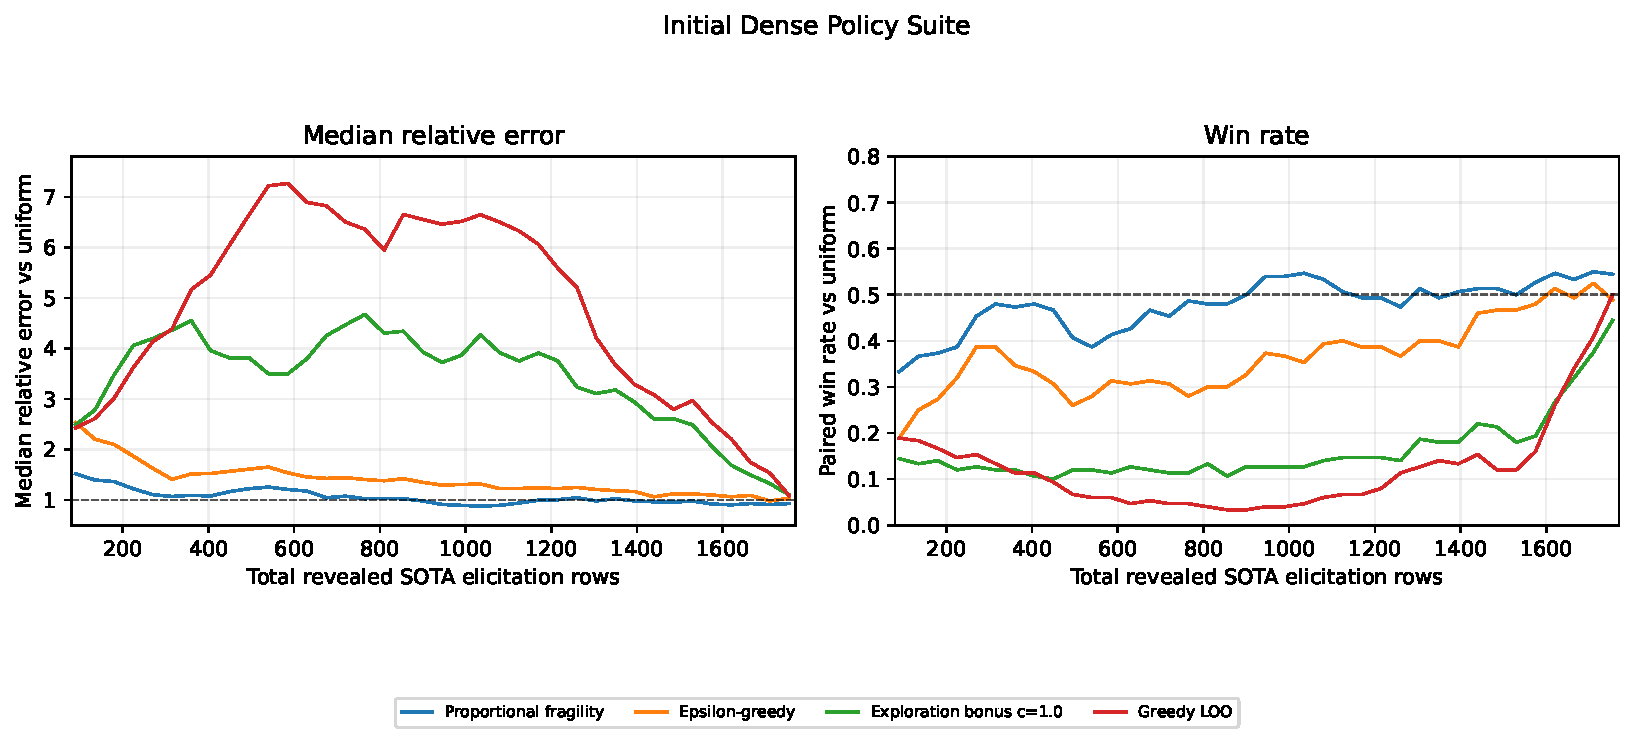
\includegraphics[width=\textwidth]{figures/results/initial_suite_smoothed_relative_error_and_win_rate.pdf}
\caption{Initial dense policy suite. Left: smoothed median seedwise relative error against step-balanced uniform. Right: smoothed paired win rate against step-balanced uniform. The dashed horizontal lines mark parity with uniform.}
\label{fig:initial-suite-relative-error}
\end{figure}

The deterministic fragility policies perform poorly. In Figure~\ref{fig:initial-suite-relative-error}, greedy LOO-fragility and exploration-bonus allocation remain well above uniform across most budgets. Greedy LOO-fragility is especially unstable: after smoothing, its median relative error is typically several times the uniform error. The exploration-bonus policy with $c=1.0$ is less extreme than pure greedy allocation, but still far from competitive in this dense run.

The main exception is \texttt{stochastic\_normalized\_fragility}, which samples among positive-fragility nodes with probability proportional to the current fragility score. This policy is much closer to uniform than the deterministic policies. Across the non-boundary budgets, its median relative error is below one at 19 of 38 budgets, and its paired win rate is at least 0.5 at 20 of 38 budgets. This is not enough to show clear dominance over uniform, but it changes the interpretation of the initial experiment: the problem is not simply that LOO fragility contains no useful signal. Rather, deterministic or too-concentrated use of that signal appears brittle.

This motivates the second experiment. If the stochastic proportional-fragility policy is the only competitive member of the initial suite, the next question is whether its useful feature is proportional weighting by raw fragility magnitude, or instead the weaker act of randomizing among nodes with positive fragility.

\subsection{Stochastic fragility ablation}

The second dense experiment keeps the same experimental settings but replaces deterministic allocation rules with stochastic variants. The policies compared here are the step-balanced uniform baseline, stochastic proportional fragility, uniform-positive fragility, stochastic epsilon-greedy fragility, and stochastic exploration-bonus variants. The most important comparison is between stochastic proportional fragility and uniform-positive fragility.

\begin{figure}[htbp]
\centering
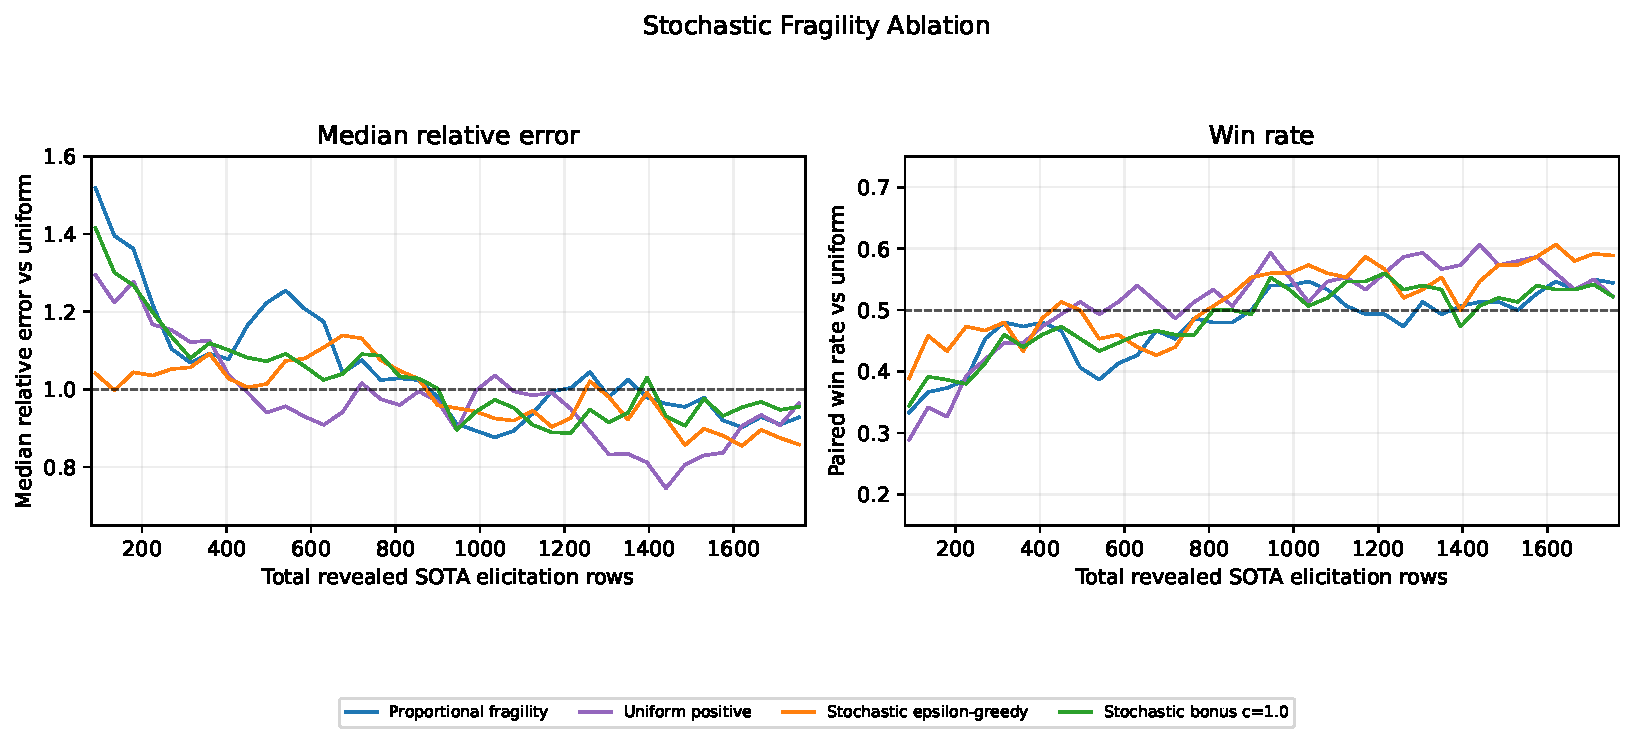
\includegraphics[width=\textwidth]{figures/results/stochastic_ablation_smoothed_relative_error_and_win_rate.pdf}
\caption{Stochastic fragility ablation. The main comparison is between proportional weighting by raw positive fragility and uniform sampling among positive-fragility nodes. Left: smoothed median seedwise relative error against step-balanced uniform. Right: smoothed paired win rate against step-balanced uniform.}
\label{fig:stochastic-ablation-relative-error}
\end{figure}

The stochasticized policies are much more competitive than the deterministic fragility policies in the initial suite. None of them uniformly dominates the step-balanced baseline at every budget, but their relative-error curves stay close to one rather than diverging by large factors.

Uniform-positive fragility is the most informative diagnostic policy in this experiment. It ignores raw fragility magnitudes after using fragility only to identify nodes with positive finite scores. Despite this simpler rule, it performs at least as well as stochastic proportional fragility in the main budget-dependent comparisons. Across the 38 non-boundary budgets, uniform-positive fragility has median relative error below one at 20 budgets and paired win rate above 0.5 at 20 budgets. Stochastic proportional fragility has median relative error below one at 19 budgets and win rate above 0.5 at 14 budgets.

The stochastic epsilon-greedy policy is also competitive, with median relative error below one at 22 of the 38 non-boundary budgets and win rate above 0.5 at 21 budgets. The stochastic exploration-bonus policy with $c=1.0$ is close to the baseline, but does not clearly improve on the simpler stochastic rules.

These results suggest that positive LOO fragility does contain useful allocation information, but that the raw magnitudes are not well calibrated as sampling probabilities. A policy that randomizes among positive-fragility nodes can perform comparably to, and in some comparisons better than, a policy that samples in direct proportion to the fragility scores.

\subsection{Softmax temperature ablation}

The third dense experiment tests whether the proportional-fragility policy can be improved by softmax temperature scaling. The motivation is that raw LOO fragility scores may rank or identify useful nodes while still being too poorly calibrated to use directly as probabilities. Softmax scaling provides a controlled way to vary the sharpness of magnitude-weighted sampling.

\begin{figure}[htbp]
\centering
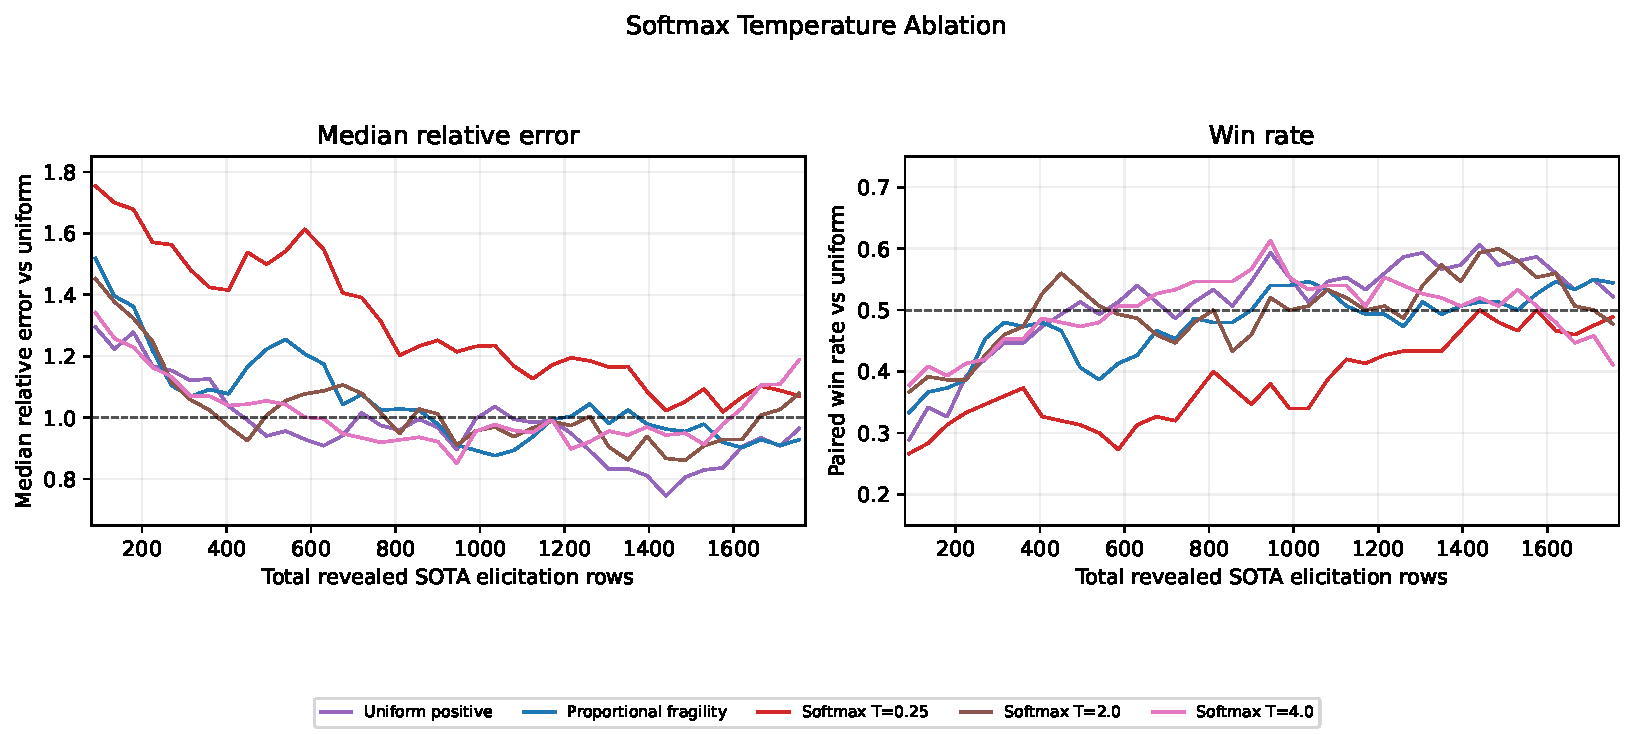
\includegraphics[width=\textwidth]{figures/results/softmax_ablation_smoothed_relative_error_and_win_rate.pdf}
\caption{Softmax temperature ablation. Lower temperatures make sampling sharper and closer to greedy selection; higher temperatures flatten the distribution over positive-fragility nodes. Left: smoothed median seedwise relative error against step-balanced uniform. Right: smoothed paired win rate against step-balanced uniform.}
\label{fig:softmax-ablation-relative-error}
\end{figure}

The softmax results support the calibration interpretation. The sharpest tested softmax policy, $T=0.25$, performs poorly: across non-boundary budgets, its median relative error is below one at only 3 of 38 budgets. In Figure~\ref{fig:softmax-ablation-relative-error}, it remains above uniform for most of the budget range. This is consistent with the failure mode seen in deterministic fragility policies: over-sharp use of a noisy fragility signal leads to over-concentration.

Flatter softmax policies are more competitive. The $T=2.0$ and $T=4.0$ variants stay much closer to uniform and to the stochastic ablation policies. The $T=4.0$ variant has median relative error below one at 20 of 38 non-boundary budgets, similar to uniform-positive fragility. However, the softmax variants do not clearly improve on the simpler uniform-positive rule. The empirical lesson is therefore not that temperature scaling solves the problem, but that reducing the sharpness of magnitude-weighted sampling helps.

Taken together, the stochastic and softmax ablations point to the same conclusion. LOO output fragility appears to identify nodes where additional elicitation can be useful, but the raw fragility magnitudes should not be treated as calibrated probabilities. The most promising policies in these experiments are those that use fragility to restrict or soften the candidate set while preserving substantial randomization.

\subsection{Summary of empirical findings}

The dense experiments support four main findings.

First, the step-balanced uniform policy is a strong baseline. This matters because the evaluation target is a full-data exchangeable reference distribution, and uniform allocation is naturally well matched to recovering nodewise mixtures when no reliable prioritization signal is available.

Second, deterministic use of LOO fragility is not competitive in this setting. Greedy and exploration-bonus policies over-concentrate allocation and often have much larger error than uniform.

Third, stochastic use of positive fragility is substantially more promising. The proportional-fragility policy from the initial suite is close enough to uniform to motivate follow-up, and the uniform-positive and stochastic epsilon-greedy ablations perform at least as well in the budget-dependent comparisons.

Fourth, softmax temperature scaling improves over very sharp magnitude-weighted sampling, but does not clearly beat the simpler uniform-positive policy. This suggests that the sign or positivity of LOO fragility is more reliable than the exact raw magnitude.

These results should be interpreted as exploratory. They do not identify an optimal allocation rule, and they do not show that fragility-guided elicitation allocation universally beats uniform allocation. They do, however, provide evidence that output-sensitive allocation is worth further study, especially through stochastic policies that avoid over-committing to noisy fragility estimates.

\section{Limitations and Future Work}

\paragraph{Restriction to OC3 Denial of Service submodel} While the risk model we used here for the experiments is helpful for an initial investigation of the utility of our methodology, ideally we would test with the other (if not all of the) risk models developed by SaferAI that were provided in (\cite{barrett2025toward}). Also, with this OC3 Denial of Service model, we did not work with the entire risk model, and therefore did not consider how well this works at recovering a similar estimate for the total-risk probability distribution to that of the full model. This introduces additional considerations, including whether we ought to work with $\log(\text{TotalRisk})$ rather than simply $\text{TotalRisk}$, since our primary objective is directional, rather than absolute, correctness.

\paragraph{Use of only SOTA inputs} Ideally, we would have performed experiments across various (if not all) potential inputs. There are many open questions in this direction. Namely, there is the question of how best to weight performance at different inputs, and how to update this weighting as time goes on and LLM capabilities improve. 

\paragraph{Assumption each expert has identical cost} The budget unit is an LLM elicitation draw, not an independent human expert, so it is already an imperfect modeling assumption. Beyond this, though, we should remember that when using real human experts, it may well be the case that it is cheaper to ``use them'' the more information they are asked to provide. We would expect this to be the case to a lesser extent with ``LLM experts'', and given the way the field is moving towards this, our assumption, while imperfect, may become less of an issue in the years to come.

\paragraph{Lack of ground truth} The full-data reference is not ground truth. This is an inherent difficulty we have whenever we are working on ways to improve quantitative AI risk modeling methodologies of this kind, but it is a limitation nonetheless. Our proposed methodology is best viewed as an attempt to produce a good output distribution with a reduced budget.

\paragraph{LOO fragility is merely an instability heuristic} While we would expect that our heuristic provides a reasonable approximation of the benefit of obtaining an additional draw for a certain node in the model, there are no guarantees that this ought to be the case. It could be possible to develop a heuristic in a more principled way, by using previous draws to give an estimate of the distribution of future probability distribution draws, and use this to form the basis of our heuristic. This would be following an approach similar to that used in Bayesian experimental design. It would likely be far more computationally expensive, so the feasibility of this remains an open question.

\paragraph{Computational limitations} The number of reveal seeds is modest and batching was used for fragility recomputation. For runtime reasons, the policy runs used approximate LOO-term subsampling with $\texttt{max\_loo\_terms\_per\_step}=20$. A separate approximation audit compared exact LOO with capped subsampling on revealed states. In that reduced audit, cap 20 preserved the exact top fragile node in all audited comparisons, had mean top-3 Jaccard approximately 0.833, and had mean Spearman rank correlation approximately 0.833. Cap 10 was noisier and was marked questionable by the audit heuristic. This supports cap 20 as a development approximation, but it is not a proof that the approximation is exact.

\section{Conclusion}
This report outlines a retrospective budget-recovery experiment for the OC3 DoS \(\psuccess\) submodel using repeated LLM elicitation draws. The results provide preliminary evidence that output-fragility-guided allocation can reduce average recovery error in some settings, but also that greedy fragility guidance can severely over-concentrate elicitation effort. Exploration bonuses reduce concentration relative to lower-exploration variants, and \(c=1.0\) looked best among the tested exploration-bonus settings in the development sensitivity run. As a result, these findings are best viewed as evidence that this problem warrants further investigation, rather than evidence that the LOO heuristic is a desirable one in its own right.

\printbibliography

\appendix

\section{Additional Tables}
\label{app:additional-tables}

\begin{scriptsize}
\begin{longtable}{llrrrrrr}
\caption{Dense policy suite by-budget metrics. Relative errors are computed within reveal seed against the step-balanced uniform baseline before averaging or taking medians across seeds.}\label{tab:dense-policy-suite-by-budget-metrics}\\
\toprule
Policy & Budget & Seeds & Mean error & Median error & Win rate & Mean rel. error & Median rel. error \\
\midrule
\endfirsthead
\toprule
Policy & Budget & Seeds & Mean error & Median error & Win rate & Mean rel. error & Median rel. error \\
\midrule
\endhead
Uniform & 45 & 30 & 4.995e-05 & 4.629e-05 & -- & 1.000 & 1.000 \\
Uniform & 90 & 30 & 2.386e-05 & 1.673e-05 & -- & 1.000 & 1.000 \\
Uniform & 135 & 30 & 1.780e-05 & 1.014e-05 & -- & 1.000 & 1.000 \\
Uniform & 180 & 30 & 1.554e-05 & 1.116e-05 & -- & 1.000 & 1.000 \\
Uniform & 225 & 30 & 1.304e-05 & 1.052e-05 & -- & 1.000 & 1.000 \\
Uniform & 270 & 30 & 9.694e-06 & 6.052e-06 & -- & 1.000 & 1.000 \\
Uniform & 315 & 30 & 9.705e-06 & 6.992e-06 & -- & 1.000 & 1.000 \\
Uniform & 360 & 30 & 1.018e-05 & 6.563e-06 & -- & 1.000 & 1.000 \\
Uniform & 405 & 30 & 7.905e-06 & 6.515e-06 & -- & 1.000 & 1.000 \\
Uniform & 450 & 30 & 7.706e-06 & 5.546e-06 & -- & 1.000 & 1.000 \\
Uniform & 495 & 30 & 6.750e-06 & 5.416e-06 & -- & 1.000 & 1.000 \\
Uniform & 540 & 30 & 5.954e-06 & 4.762e-06 & -- & 1.000 & 1.000 \\
Uniform & 585 & 30 & 5.411e-06 & 4.703e-06 & -- & 1.000 & 1.000 \\
Uniform & 630 & 30 & 5.416e-06 & 5.245e-06 & -- & 1.000 & 1.000 \\
Uniform & 675 & 30 & 5.474e-06 & 4.572e-06 & -- & 1.000 & 1.000 \\
Uniform & 720 & 30 & 5.774e-06 & 4.769e-06 & -- & 1.000 & 1.000 \\
Uniform & 765 & 30 & 5.230e-06 & 4.900e-06 & -- & 1.000 & 1.000 \\
Uniform & 810 & 30 & 4.221e-06 & 4.539e-06 & -- & 1.000 & 1.000 \\
Uniform & 855 & 30 & 4.689e-06 & 3.946e-06 & -- & 1.000 & 1.000 \\
Uniform & 900 & 30 & 5.681e-06 & 4.335e-06 & -- & 1.000 & 1.000 \\
Uniform & 945 & 30 & 3.400e-06 & 2.579e-06 & -- & 1.000 & 1.000 \\
Uniform & 990 & 30 & 3.849e-06 & 3.315e-06 & -- & 1.000 & 1.000 \\
Uniform & 1035 & 30 & 4.932e-06 & 3.973e-06 & -- & 1.000 & 1.000 \\
Uniform & 1080 & 30 & 3.511e-06 & 2.501e-06 & -- & 1.000 & 1.000 \\
Uniform & 1125 & 30 & 3.657e-06 & 3.213e-06 & -- & 1.000 & 1.000 \\
Uniform & 1170 & 30 & 3.717e-06 & 2.891e-06 & -- & 1.000 & 1.000 \\
Uniform & 1215 & 30 & 4.283e-06 & 3.172e-06 & -- & 1.000 & 1.000 \\
Uniform & 1260 & 30 & 3.305e-06 & 3.052e-06 & -- & 1.000 & 1.000 \\
Uniform & 1305 & 30 & 3.024e-06 & 2.590e-06 & -- & 1.000 & 1.000 \\
Uniform & 1350 & 30 & 3.247e-06 & 3.037e-06 & -- & 1.000 & 1.000 \\
Uniform & 1395 & 30 & 4.936e-06 & 3.499e-06 & -- & 1.000 & 1.000 \\
Uniform & 1440 & 30 & 4.181e-06 & 2.521e-06 & -- & 1.000 & 1.000 \\
Uniform & 1485 & 30 & 2.881e-06 & 2.466e-06 & -- & 1.000 & 1.000 \\
Uniform & 1530 & 30 & 3.812e-06 & 3.047e-06 & -- & 1.000 & 1.000 \\
Uniform & 1575 & 30 & 2.853e-06 & 2.310e-06 & -- & 1.000 & 1.000 \\
Uniform & 1620 & 30 & 3.231e-06 & 2.577e-06 & -- & 1.000 & 1.000 \\
Uniform & 1665 & 30 & 3.157e-06 & 2.679e-06 & -- & 1.000 & 1.000 \\
Uniform & 1710 & 30 & 2.915e-06 & 2.324e-06 & -- & 1.000 & 1.000 \\
Uniform & 1755 & 30 & 2.705e-06 & 2.359e-06 & -- & 1.000 & 1.000 \\
Uniform & 1798 & 30 & 0.000e+00 & 0.000e+00 & -- & -- & -- \\
Stoch proportional & 45 & 30 & 4.995e-05 & 4.629e-05 & 0.000 & 1.000 & 1.000 \\
Stoch proportional & 90 & 30 & 3.842e-05 & 3.108e-05 & 0.333 & 2.138 & 1.886 \\
Stoch proportional & 135 & 30 & 2.633e-05 & 1.816e-05 & 0.333 & 2.488 & 1.423 \\
Stoch proportional & 180 & 30 & 2.315e-05 & 1.836e-05 & 0.333 & 2.285 & 1.248 \\
Stoch proportional & 225 & 30 & 1.462e-05 & 9.414e-06 & 0.467 & 1.314 & 1.026 \\
Stoch proportional & 270 & 30 & 1.107e-05 & 7.261e-06 & 0.400 & 1.327 & 1.227 \\
Stoch proportional & 315 & 30 & 9.645e-06 & 7.593e-06 & 0.400 & 1.407 & 1.174 \\
Stoch proportional & 360 & 30 & 9.106e-06 & 6.814e-06 & 0.667 & 1.193 & 0.847 \\
Stoch proportional & 405 & 30 & 9.387e-06 & 6.769e-06 & 0.467 & 1.266 & 1.069 \\
Stoch proportional & 450 & 30 & 8.542e-06 & 6.126e-06 & 0.433 & 1.341 & 1.143 \\
Stoch proportional & 495 & 30 & 7.532e-06 & 6.500e-06 & 0.433 & 1.394 & 1.155 \\
Stoch proportional & 540 & 30 & 7.299e-06 & 5.980e-06 & 0.333 & 1.617 & 1.612 \\
Stoch proportional & 585 & 30 & 6.177e-06 & 5.838e-06 & 0.367 & 1.280 & 1.135 \\
Stoch proportional & 630 & 30 & 6.026e-06 & 5.057e-06 & 0.367 & 1.262 & 1.228 \\
Stoch proportional & 675 & 30 & 5.091e-06 & 3.883e-06 & 0.567 & 1.108 & 0.908 \\
Stoch proportional & 720 & 30 & 5.337e-06 & 4.824e-06 & 0.500 & 1.176 & 0.990 \\
Stoch proportional & 765 & 30 & 4.645e-06 & 3.566e-06 & 0.533 & 1.326 & 0.954 \\
Stoch proportional & 810 & 30 & 5.827e-06 & 4.853e-06 & 0.300 & 1.839 & 1.296 \\
Stoch proportional & 855 & 30 & 4.698e-06 & 4.727e-06 & 0.533 & 1.146 & 0.972 \\
Stoch proportional & 900 & 30 & 4.704e-06 & 3.650e-06 & 0.533 & 1.045 & 0.929 \\
Stoch proportional & 945 & 30 & 3.395e-06 & 3.081e-06 & 0.500 & 1.295 & 0.968 \\
Stoch proportional & 990 & 30 & 3.293e-06 & 3.251e-06 & 0.633 & 1.090 & 0.734 \\
Stoch proportional & 1035 & 30 & 4.272e-06 & 2.610e-06 & 0.500 & 1.092 & 0.951 \\
Stoch proportional & 1080 & 30 & 3.334e-06 & 2.716e-06 & 0.533 & 1.410 & 0.885 \\
Stoch proportional & 1125 & 30 & 3.810e-06 & 2.928e-06 & 0.567 & 1.534 & 0.842 \\
Stoch proportional & 1170 & 30 & 3.912e-06 & 2.769e-06 & 0.433 & 1.377 & 1.054 \\
Stoch proportional & 1215 & 30 & 4.771e-06 & 3.341e-06 & 0.500 & 2.000 & 0.957 \\
Stoch proportional & 1260 & 30 & 4.175e-06 & 2.555e-06 & 0.433 & 1.933 & 1.237 \\
Stoch proportional & 1305 & 30 & 3.674e-06 & 2.728e-06 & 0.533 & 1.621 & 0.928 \\
Stoch proportional & 1350 & 30 & 2.992e-06 & 2.365e-06 & 0.467 & 1.200 & 1.048 \\
Stoch proportional & 1395 & 30 & 3.170e-06 & 2.376e-06 & 0.633 & 1.202 & 0.734 \\
Stoch proportional & 1440 & 30 & 3.418e-06 & 2.912e-06 & 0.400 & 1.543 & 1.177 \\
Stoch proportional & 1485 & 30 & 3.234e-06 & 2.651e-06 & 0.500 & 1.238 & 1.010 \\
Stoch proportional & 1530 & 30 & 3.022e-06 & 2.375e-06 & 0.567 & 1.215 & 0.845 \\
Stoch proportional & 1575 & 30 & 3.211e-06 & 2.411e-06 & 0.467 & 1.313 & 1.008 \\
Stoch proportional & 1620 & 30 & 3.178e-06 & 2.089e-06 & 0.567 & 1.105 & 0.853 \\
Stoch proportional & 1665 & 30 & 2.990e-06 & 2.278e-06 & 0.533 & 1.223 & 0.882 \\
Stoch proportional & 1710 & 30 & 2.373e-06 & 1.906e-06 & 0.600 & 1.334 & 0.923 \\
Stoch proportional & 1755 & 30 & 2.331e-06 & 1.862e-06 & 0.500 & 1.251 & 0.979 \\
Stoch proportional & 1798 & 30 & 0.000e+00 & 0.000e+00 & 0.000 & -- & -- \\
Eps-greedy 0.2 & 45 & 30 & 4.995e-05 & 4.629e-05 & 0.000 & 1.000 & 1.000 \\
Eps-greedy 0.2 & 90 & 30 & 6.066e-05 & 5.646e-05 & 0.133 & 3.930 & 2.677 \\
Eps-greedy 0.2 & 135 & 30 & 4.860e-05 & 3.607e-05 & 0.133 & 4.561 & 2.433 \\
Eps-greedy 0.2 & 180 & 30 & 2.954e-05 & 2.513e-05 & 0.300 & 4.336 & 2.487 \\
Eps-greedy 0.2 & 225 & 30 & 2.149e-05 & 1.685e-05 & 0.433 & 2.404 & 1.218 \\
Eps-greedy 0.2 & 270 & 30 & 1.687e-05 & 1.277e-05 & 0.367 & 3.329 & 1.671 \\
Eps-greedy 0.2 & 315 & 30 & 1.605e-05 & 1.109e-05 & 0.367 & 2.950 & 1.520 \\
Eps-greedy 0.2 & 360 & 30 & 1.421e-05 & 9.869e-06 & 0.467 & 2.009 & 1.243 \\
Eps-greedy 0.2 & 405 & 30 & 1.228e-05 & 7.209e-06 & 0.300 & 1.763 & 1.390 \\
Eps-greedy 0.2 & 450 & 30 & 1.216e-05 & 1.112e-05 & 0.233 & 2.155 & 1.755 \\
Eps-greedy 0.2 & 495 & 30 & 1.118e-05 & 9.324e-06 & 0.300 & 2.422 & 1.712 \\
Eps-greedy 0.2 & 540 & 30 & 9.161e-06 & 7.874e-06 & 0.233 & 2.173 & 1.737 \\
Eps-greedy 0.2 & 585 & 30 & 9.856e-06 & 6.599e-06 & 0.233 & 2.010 & 1.458 \\
Eps-greedy 0.2 & 630 & 30 & 9.032e-06 & 6.877e-06 & 0.400 & 2.329 & 1.594 \\
Eps-greedy 0.2 & 675 & 30 & 7.607e-06 & 5.312e-06 & 0.400 & 2.252 & 1.188 \\
Eps-greedy 0.2 & 720 & 30 & 8.310e-06 & 7.967e-06 & 0.267 & 1.963 & 1.292 \\
Eps-greedy 0.2 & 765 & 30 & 8.117e-06 & 6.198e-06 & 0.267 & 2.256 & 1.603 \\
Eps-greedy 0.2 & 810 & 30 & 7.688e-06 & 6.854e-06 & 0.200 & 2.541 & 1.528 \\
Eps-greedy 0.2 & 855 & 30 & 7.335e-06 & 5.423e-06 & 0.267 & 1.829 & 1.409 \\
Eps-greedy 0.2 & 900 & 30 & 6.587e-06 & 5.630e-06 & 0.500 & 1.589 & 1.068 \\
Eps-greedy 0.2 & 945 & 30 & 6.273e-06 & 3.873e-06 & 0.267 & 2.204 & 1.497 \\
Eps-greedy 0.2 & 990 & 30 & 4.950e-06 & 3.611e-06 & 0.400 & 1.594 & 1.243 \\
Eps-greedy 0.2 & 1035 & 30 & 5.543e-06 & 4.613e-06 & 0.433 & 1.662 & 1.251 \\
Eps-greedy 0.2 & 1080 & 30 & 5.018e-06 & 3.969e-06 & 0.233 & 2.224 & 1.471 \\
Eps-greedy 0.2 & 1125 & 30 & 4.137e-06 & 4.051e-06 & 0.433 & 1.692 & 1.116 \\
Eps-greedy 0.2 & 1170 & 30 & 4.106e-06 & 3.240e-06 & 0.467 & 1.679 & 1.032 \\
Eps-greedy 0.2 & 1215 & 30 & 4.903e-06 & 3.943e-06 & 0.433 & 1.742 & 1.270 \\
Eps-greedy 0.2 & 1260 & 30 & 4.677e-06 & 3.981e-06 & 0.367 & 1.860 & 1.305 \\
Eps-greedy 0.2 & 1305 & 30 & 4.742e-06 & 4.288e-06 & 0.233 & 2.231 & 1.405 \\
Eps-greedy 0.2 & 1350 & 30 & 4.668e-06 & 4.675e-06 & 0.333 & 2.009 & 1.223 \\
Eps-greedy 0.2 & 1395 & 30 & 3.498e-06 & 2.356e-06 & 0.633 & 1.224 & 0.836 \\
Eps-greedy 0.2 & 1440 & 30 & 4.749e-06 & 3.301e-06 & 0.433 & 2.478 & 1.143 \\
Eps-greedy 0.2 & 1485 & 30 & 3.729e-06 & 3.087e-06 & 0.300 & 1.605 & 1.222 \\
Eps-greedy 0.2 & 1530 & 30 & 4.261e-06 & 3.848e-06 & 0.600 & 1.636 & 0.884 \\
Eps-greedy 0.2 & 1575 & 30 & 4.092e-06 & 2.609e-06 & 0.367 & 1.959 & 1.523 \\
Eps-greedy 0.2 & 1620 & 30 & 2.802e-06 & 2.371e-06 & 0.633 & 1.096 & 0.826 \\
Eps-greedy 0.2 & 1665 & 30 & 3.552e-06 & 2.422e-06 & 0.500 & 1.612 & 1.032 \\
Eps-greedy 0.2 & 1710 & 30 & 3.024e-06 & 2.632e-06 & 0.467 & 1.554 & 1.049 \\
Eps-greedy 0.2 & 1755 & 30 & 3.175e-06 & 2.016e-06 & 0.500 & 1.787 & 1.016 \\
Eps-greedy 0.2 & 1798 & 30 & 0.000e+00 & 0.000e+00 & 0.000 & -- & -- \\
Bonus c=1.0 & 45 & 30 & 4.995e-05 & 4.629e-05 & 0.000 & 1.000 & 1.000 \\
Bonus c=1.0 & 90 & 30 & 4.806e-05 & 3.132e-05 & 0.233 & 3.082 & 1.709 \\
Bonus c=1.0 & 135 & 30 & 5.390e-05 & 5.647e-05 & 0.067 & 5.295 & 2.547 \\
Bonus c=1.0 & 180 & 30 & 4.485e-05 & 4.433e-05 & 0.133 & 8.792 & 3.209 \\
Bonus c=1.0 & 225 & 30 & 4.425e-05 & 3.727e-05 & 0.100 & 4.868 & 3.653 \\
Bonus c=1.0 & 270 & 30 & 4.013e-05 & 3.150e-05 & 0.167 & 8.209 & 6.276 \\
Bonus c=1.0 & 315 & 30 & 3.689e-05 & 2.611e-05 & 0.133 & 6.203 & 4.623 \\
Bonus c=1.0 & 360 & 30 & 3.416e-05 & 3.206e-05 & 0.100 & 6.065 & 3.213 \\
Bonus c=1.0 & 405 & 30 & 3.451e-05 & 2.818e-05 & 0.100 & 5.526 & 4.049 \\
Bonus c=1.0 & 450 & 30 & 3.523e-05 & 3.083e-05 & 0.100 & 7.075 & 4.579 \\
Bonus c=1.0 & 495 & 30 & 3.262e-05 & 2.621e-05 & 0.100 & 8.507 & 3.314 \\
Bonus c=1.0 & 540 & 30 & 3.027e-05 & 2.054e-05 & 0.100 & 10.308 & 3.891 \\
Bonus c=1.0 & 585 & 30 & 2.982e-05 & 1.389e-05 & 0.200 & 6.929 & 3.235 \\
Bonus c=1.0 & 630 & 30 & 2.638e-05 & 1.310e-05 & 0.100 & 5.912 & 2.479 \\
Bonus c=1.0 & 675 & 30 & 2.699e-05 & 1.382e-05 & 0.067 & 6.650 & 4.554 \\
Bonus c=1.0 & 720 & 30 & 2.891e-05 & 1.801e-05 & 0.167 & 7.416 & 4.834 \\
Bonus c=1.0 & 765 & 30 & 2.738e-05 & 1.533e-05 & 0.067 & 8.063 & 6.160 \\
Bonus c=1.0 & 810 & 30 & 2.519e-05 & 1.426e-05 & 0.167 & 8.626 & 4.310 \\
Bonus c=1.0 & 855 & 30 & 2.752e-05 & 1.831e-05 & 0.100 & 8.028 & 3.504 \\
Bonus c=1.0 & 900 & 30 & 2.346e-05 & 1.354e-05 & 0.167 & 6.167 & 2.707 \\
Bonus c=1.0 & 945 & 30 & 2.271e-05 & 1.471e-05 & 0.033 & 8.627 & 5.021 \\
Bonus c=1.0 & 990 & 30 & 1.976e-05 & 1.239e-05 & 0.167 & 6.182 & 4.122 \\
Bonus c=1.0 & 1035 & 30 & 1.928e-05 & 1.113e-05 & 0.167 & 6.050 & 3.260 \\
Bonus c=1.0 & 1080 & 30 & 2.044e-05 & 1.156e-05 & 0.100 & 12.253 & 4.207 \\
Bonus c=1.0 & 1125 & 30 & 2.027e-05 & 1.310e-05 & 0.167 & 7.210 & 4.737 \\
Bonus c=1.0 & 1170 & 30 & 1.841e-05 & 7.945e-06 & 0.100 & 6.091 & 3.244 \\
Bonus c=1.0 & 1215 & 30 & 1.559e-05 & 8.031e-06 & 0.200 & 5.873 & 3.310 \\
Bonus c=1.0 & 1260 & 30 & 1.720e-05 & 9.597e-06 & 0.167 & 8.921 & 4.037 \\
Bonus c=1.0 & 1305 & 30 & 1.285e-05 & 8.291e-06 & 0.100 & 6.371 & 3.454 \\
Bonus c=1.0 & 1350 & 30 & 9.962e-06 & 7.447e-06 & 0.133 & 3.945 & 2.132 \\
Bonus c=1.0 & 1395 & 30 & 1.078e-05 & 9.420e-06 & 0.333 & 5.216 & 2.606 \\
Bonus c=1.0 & 1440 & 30 & 1.130e-05 & 9.076e-06 & 0.167 & 5.098 & 3.659 \\
Bonus c=1.0 & 1485 & 30 & 9.328e-06 & 6.565e-06 & 0.167 & 3.844 & 2.812 \\
Bonus c=1.0 & 1530 & 30 & 6.840e-06 & 5.512e-06 & 0.300 & 3.072 & 1.797 \\
Bonus c=1.0 & 1575 & 30 & 6.694e-06 & 4.866e-06 & 0.100 & 2.955 & 2.166 \\
Bonus c=1.0 & 1620 & 30 & 6.768e-06 & 5.571e-06 & 0.167 & 2.313 & 1.998 \\
Bonus c=1.0 & 1665 & 30 & 4.998e-06 & 4.302e-06 & 0.233 & 1.950 & 1.532 \\
Bonus c=1.0 & 1710 & 30 & 2.742e-06 & 2.471e-06 & 0.533 & 1.568 & 0.952 \\
Bonus c=1.0 & 1755 & 30 & 3.115e-06 & 2.364e-06 & 0.567 & 1.898 & 0.820 \\
Bonus c=1.0 & 1798 & 30 & 0.000e+00 & 0.000e+00 & 0.000 & -- & -- \\
Greedy LOO & 45 & 30 & 4.995e-05 & 4.629e-05 & 0.000 & 1.000 & 1.000 \\
Greedy LOO & 90 & 30 & 4.593e-05 & 3.290e-05 & 0.233 & 2.765 & 2.035 \\
Greedy LOO & 135 & 30 & 4.718e-05 & 3.747e-05 & 0.167 & 4.154 & 2.426 \\
Greedy LOO & 180 & 30 & 4.406e-05 & 2.992e-05 & 0.167 & 5.559 & 2.808 \\
Greedy LOO & 225 & 30 & 4.604e-05 & 3.121e-05 & 0.167 & 5.569 & 3.178 \\
Greedy LOO & 270 & 30 & 4.427e-05 & 3.409e-05 & 0.100 & 9.662 & 4.635 \\
Greedy LOO & 315 & 30 & 4.280e-05 & 3.045e-05 & 0.133 & 7.147 & 5.082 \\
Greedy LOO & 360 & 30 & 4.277e-05 & 2.882e-05 & 0.200 & 7.507 & 4.971 \\
Greedy LOO & 405 & 30 & 4.350e-05 & 3.394e-05 & 0.067 & 8.189 & 4.057 \\
Greedy LOO & 450 & 30 & 4.817e-05 & 3.553e-05 & 0.067 & 10.011 & 7.085 \\
Greedy LOO & 495 & 30 & 4.515e-05 & 2.942e-05 & 0.100 & 10.303 & 6.072 \\
Greedy LOO & 540 & 30 & 4.402e-05 & 3.009e-05 & 0.033 & 11.119 & 8.095 \\
Greedy LOO & 585 & 30 & 4.344e-05 & 2.911e-05 & 0.067 & 9.426 & 7.934 \\
Greedy LOO & 630 & 30 & 4.437e-05 & 3.124e-05 & 0.033 & 10.159 & 6.906 \\
Greedy LOO & 675 & 30 & 3.799e-05 & 2.090e-05 & 0.067 & 12.567 & 7.334 \\
Greedy LOO & 720 & 30 & 3.862e-05 & 2.432e-05 & 0.033 & 13.021 & 4.187 \\
Greedy LOO & 765 & 30 & 3.728e-05 & 2.098e-05 & 0.067 & 12.495 & 7.764 \\
Greedy LOO & 810 & 30 & 3.649e-05 & 2.371e-05 & 0.033 & 14.850 & 6.322 \\
Greedy LOO & 855 & 30 & 3.888e-05 & 2.329e-05 & 0.033 & 9.975 & 6.187 \\
Greedy LOO & 900 & 30 & 3.746e-05 & 2.142e-05 & 0.033 & 9.880 & 5.274 \\
Greedy LOO & 945 & 30 & 3.567e-05 & 1.744e-05 & 0.000 & 12.896 & 7.720 \\
Greedy LOO & 990 & 30 & 3.606e-05 & 1.791e-05 & 0.067 & 11.741 & 7.273 \\
Greedy LOO & 1035 & 30 & 3.159e-05 & 1.633e-05 & 0.067 & 10.296 & 5.849 \\
Greedy LOO & 1080 & 30 & 2.529e-05 & 1.475e-05 & 0.033 & 13.932 & 6.459 \\
Greedy LOO & 1125 & 30 & 2.694e-05 & 1.915e-05 & 0.067 & 8.964 & 5.936 \\
Greedy LOO & 1170 & 30 & 2.621e-05 & 1.472e-05 & 0.067 & 10.334 & 6.981 \\
Greedy LOO & 1215 & 30 & 2.725e-05 & 2.014e-05 & 0.100 & 9.435 & 6.403 \\
Greedy LOO & 1260 & 30 & 1.625e-05 & 1.332e-05 & 0.067 & 6.098 & 4.540 \\
Greedy LOO & 1305 & 30 & 1.313e-05 & 1.179e-05 & 0.100 & 5.903 & 4.105 \\
Greedy LOO & 1350 & 30 & 1.217e-05 & 8.105e-06 & 0.233 & 5.394 & 4.010 \\
Greedy LOO & 1395 & 30 & 1.202e-05 & 8.696e-06 & 0.133 & 3.779 & 1.994 \\
Greedy LOO & 1440 & 30 & 1.262e-05 & 8.472e-06 & 0.167 & 5.611 & 3.693 \\
Greedy LOO & 1485 & 30 & 1.169e-05 & 6.836e-06 & 0.033 & 6.232 & 2.611 \\
Greedy LOO & 1530 & 30 & 1.196e-05 & 7.482e-06 & 0.200 & 6.369 & 3.099 \\
Greedy LOO & 1575 & 30 & 1.188e-05 & 7.001e-06 & 0.067 & 5.903 & 2.568 \\
Greedy LOO & 1620 & 30 & 9.968e-06 & 7.934e-06 & 0.133 & 4.032 & 2.873 \\
Greedy LOO & 1665 & 30 & 4.345e-06 & 3.800e-06 & 0.367 & 1.773 & 1.526 \\
Greedy LOO & 1710 & 30 & 2.837e-06 & 2.500e-06 & 0.533 & 1.594 & 0.973 \\
Greedy LOO & 1755 & 30 & 3.089e-06 & 2.364e-06 & 0.600 & 1.839 & 0.768 \\
Greedy LOO & 1798 & 30 & 0.000e+00 & 0.000e+00 & 0.000 & -- & -- \\
Bonus c=0.5 & 45 & 30 & 4.995e-05 & 4.629e-05 & 0.000 & 1.000 & 1.000 \\
Bonus c=0.5 & 90 & 30 & 5.079e-05 & 4.062e-05 & 0.200 & 3.401 & 1.818 \\
Bonus c=0.5 & 135 & 30 & 4.870e-05 & 3.469e-05 & 0.100 & 3.995 & 2.880 \\
Bonus c=0.5 & 180 & 30 & 4.797e-05 & 3.233e-05 & 0.100 & 5.819 & 3.466 \\
Bonus c=0.5 & 225 & 30 & 4.959e-05 & 3.181e-05 & 0.067 & 5.473 & 3.747 \\
Bonus c=0.5 & 270 & 30 & 4.211e-05 & 2.541e-05 & 0.033 & 6.865 & 4.517 \\
Bonus c=0.5 & 315 & 30 & 4.842e-05 & 3.202e-05 & 0.100 & 8.327 & 4.448 \\
Bonus c=0.5 & 360 & 30 & 4.113e-05 & 3.547e-05 & 0.133 & 7.173 & 4.361 \\
Bonus c=0.5 & 405 & 30 & 4.247e-05 & 3.678e-05 & 0.033 & 7.615 & 4.723 \\
Bonus c=0.5 & 450 & 30 & 4.540e-05 & 3.721e-05 & 0.033 & 9.736 & 7.773 \\
Bonus c=0.5 & 495 & 30 & 4.682e-05 & 3.520e-05 & 0.000 & 12.085 & 5.305 \\
Bonus c=0.5 & 540 & 30 & 4.237e-05 & 3.527e-05 & 0.033 & 12.616 & 7.700 \\
Bonus c=0.5 & 585 & 30 & 4.092e-05 & 3.197e-05 & 0.000 & 10.167 & 5.249 \\
Bonus c=0.5 & 630 & 30 & 3.908e-05 & 2.754e-05 & 0.033 & 9.374 & 4.774 \\
Bonus c=0.5 & 675 & 30 & 4.157e-05 & 3.036e-05 & 0.033 & 10.157 & 6.854 \\
Bonus c=0.5 & 720 & 30 & 3.810e-05 & 2.299e-05 & 0.100 & 10.083 & 4.759 \\
Bonus c=0.5 & 765 & 30 & 3.653e-05 & 2.352e-05 & 0.033 & 13.707 & 6.266 \\
Bonus c=0.5 & 810 & 30 & 3.677e-05 & 2.175e-05 & 0.000 & 12.361 & 6.356 \\
Bonus c=0.5 & 855 & 30 & 3.870e-05 & 2.476e-05 & 0.000 & 12.112 & 6.126 \\
Bonus c=0.5 & 900 & 30 & 3.528e-05 & 2.034e-05 & 0.067 & 11.158 & 4.693 \\
Bonus c=0.5 & 945 & 30 & 3.401e-05 & 1.919e-05 & 0.033 & 12.921 & 8.044 \\
Bonus c=0.5 & 990 & 30 & 3.314e-05 & 1.998e-05 & 0.033 & 12.168 & 5.384 \\
Bonus c=0.5 & 1035 & 30 & 3.260e-05 & 2.582e-05 & 0.133 & 10.588 & 6.168 \\
Bonus c=0.5 & 1080 & 30 & 2.656e-05 & 1.793e-05 & 0.067 & 13.291 & 6.400 \\
Bonus c=0.5 & 1125 & 30 & 2.871e-05 & 1.973e-05 & 0.033 & 15.020 & 6.446 \\
Bonus c=0.5 & 1170 & 30 & 2.690e-05 & 1.718e-05 & 0.100 & 10.989 & 6.552 \\
Bonus c=0.5 & 1215 & 30 & 2.831e-05 & 1.730e-05 & 0.067 & 12.864 & 5.040 \\
Bonus c=0.5 & 1260 & 30 & 2.627e-05 & 1.713e-05 & 0.000 & 12.436 & 4.998 \\
Bonus c=0.5 & 1305 & 30 & 2.331e-05 & 1.619e-05 & 0.067 & 11.676 & 5.626 \\
Bonus c=0.5 & 1350 & 30 & 2.348e-05 & 1.487e-05 & 0.100 & 10.491 & 5.082 \\
Bonus c=0.5 & 1395 & 30 & 2.400e-05 & 1.487e-05 & 0.067 & 13.751 & 2.770 \\
Bonus c=0.5 & 1440 & 30 & 2.216e-05 & 1.486e-05 & 0.033 & 9.079 & 4.850 \\
Bonus c=0.5 & 1485 & 30 & 2.071e-05 & 1.289e-05 & 0.133 & 9.599 & 6.111 \\
Bonus c=0.5 & 1530 & 30 & 1.728e-05 & 1.044e-05 & 0.100 & 7.818 & 3.265 \\
Bonus c=0.5 & 1575 & 30 & 1.727e-05 & 9.795e-06 & 0.100 & 9.366 & 3.662 \\
Bonus c=0.5 & 1620 & 30 & 8.219e-06 & 6.901e-06 & 0.033 & 3.103 & 2.279 \\
Bonus c=0.5 & 1665 & 30 & 4.967e-06 & 4.209e-06 & 0.300 & 2.029 & 1.613 \\
Bonus c=0.5 & 1710 & 30 & 2.860e-06 & 2.500e-06 & 0.533 & 1.600 & 0.987 \\
Bonus c=0.5 & 1755 & 30 & 3.108e-06 & 2.364e-06 & 0.567 & 1.873 & 0.820 \\
Bonus c=0.5 & 1798 & 30 & 0.000e+00 & 0.000e+00 & 0.000 & -- & -- \\
Bonus c=0.25 & 45 & 30 & 4.995e-05 & 4.629e-05 & 0.000 & 1.000 & 1.000 \\
Bonus c=0.25 & 90 & 30 & 4.873e-05 & 4.309e-05 & 0.200 & 3.094 & 1.854 \\
Bonus c=0.25 & 135 & 30 & 4.949e-05 & 4.036e-05 & 0.100 & 4.380 & 3.222 \\
Bonus c=0.25 & 180 & 30 & 4.518e-05 & 3.724e-05 & 0.167 & 5.354 & 3.139 \\
Bonus c=0.25 & 225 & 30 & 4.710e-05 & 4.099e-05 & 0.133 & 6.619 & 4.204 \\
Bonus c=0.25 & 270 & 30 & 4.524e-05 & 3.767e-05 & 0.133 & 9.962 & 5.341 \\
Bonus c=0.25 & 315 & 30 & 4.472e-05 & 3.581e-05 & 0.100 & 7.302 & 5.126 \\
Bonus c=0.25 & 360 & 30 & 4.706e-05 & 3.278e-05 & 0.167 & 8.980 & 5.075 \\
Bonus c=0.25 & 405 & 30 & 4.512e-05 & 3.418e-05 & 0.100 & 8.704 & 6.369 \\
Bonus c=0.25 & 450 & 30 & 4.779e-05 & 3.303e-05 & 0.067 & 10.307 & 6.846 \\
Bonus c=0.25 & 495 & 30 & 4.622e-05 & 3.298e-05 & 0.067 & 11.828 & 8.949 \\
Bonus c=0.25 & 540 & 30 & 4.500e-05 & 3.423e-05 & 0.100 & 13.616 & 7.337 \\
Bonus c=0.25 & 585 & 30 & 4.896e-05 & 3.495e-05 & 0.033 & 11.143 & 8.660 \\
Bonus c=0.25 & 630 & 30 & 4.386e-05 & 3.037e-05 & 0.000 & 9.515 & 7.552 \\
Bonus c=0.25 & 675 & 30 & 3.947e-05 & 2.719e-05 & 0.033 & 10.347 & 6.164 \\
Bonus c=0.25 & 720 & 30 & 4.189e-05 & 3.260e-05 & 0.000 & 10.649 & 6.863 \\
Bonus c=0.25 & 765 & 30 & 4.119e-05 & 2.755e-05 & 0.033 & 13.696 & 7.553 \\
Bonus c=0.25 & 810 & 30 & 3.920e-05 & 2.896e-05 & 0.000 & 13.937 & 7.381 \\
Bonus c=0.25 & 855 & 30 & 4.042e-05 & 2.917e-05 & 0.000 & 11.039 & 7.134 \\
Bonus c=0.25 & 900 & 30 & 3.661e-05 & 2.617e-05 & 0.100 & 11.147 & 6.916 \\
Bonus c=0.25 & 945 & 30 & 3.660e-05 & 2.043e-05 & 0.033 & 14.930 & 7.658 \\
Bonus c=0.25 & 990 & 30 & 3.591e-05 & 2.584e-05 & 0.067 & 12.394 & 7.891 \\
Bonus c=0.25 & 1035 & 30 & 3.225e-05 & 2.503e-05 & 0.100 & 10.834 & 6.794 \\
Bonus c=0.25 & 1080 & 30 & 3.402e-05 & 2.696e-05 & 0.033 & 19.614 & 9.225 \\
Bonus c=0.25 & 1125 & 30 & 3.318e-05 & 2.296e-05 & 0.033 & 11.216 & 7.988 \\
Bonus c=0.25 & 1170 & 30 & 2.929e-05 & 1.884e-05 & 0.133 & 11.743 & 8.925 \\
Bonus c=0.25 & 1215 & 30 & 3.298e-05 & 2.239e-05 & 0.100 & 12.126 & 8.197 \\
Bonus c=0.25 & 1260 & 30 & 2.592e-05 & 1.731e-05 & 0.067 & 12.087 & 6.988 \\
Bonus c=0.25 & 1305 & 30 & 2.076e-05 & 1.244e-05 & 0.067 & 9.175 & 5.370 \\
Bonus c=0.25 & 1350 & 30 & 2.139e-05 & 1.516e-05 & 0.100 & 9.392 & 6.753 \\
Bonus c=0.25 & 1395 & 30 & 1.962e-05 & 1.352e-05 & 0.133 & 7.550 & 4.188 \\
Bonus c=0.25 & 1440 & 30 & 2.044e-05 & 1.046e-05 & 0.100 & 8.807 & 5.416 \\
Bonus c=0.25 & 1485 & 30 & 1.750e-05 & 1.111e-05 & 0.000 & 11.095 & 3.633 \\
Bonus c=0.25 & 1530 & 30 & 1.844e-05 & 1.223e-05 & 0.167 & 9.098 & 5.375 \\
Bonus c=0.25 & 1575 & 30 & 1.694e-05 & 1.035e-05 & 0.033 & 11.008 & 4.033 \\
Bonus c=0.25 & 1620 & 30 & 1.129e-05 & 8.388e-06 & 0.067 & 4.480 & 3.279 \\
Bonus c=0.25 & 1665 & 30 & 4.624e-06 & 3.800e-06 & 0.333 & 1.798 & 1.596 \\
Bonus c=0.25 & 1710 & 30 & 2.837e-06 & 2.500e-06 & 0.533 & 1.594 & 0.973 \\
Bonus c=0.25 & 1755 & 30 & 3.089e-06 & 2.364e-06 & 0.600 & 1.839 & 0.768 \\
Bonus c=0.25 & 1798 & 30 & 0.000e+00 & 0.000e+00 & 0.000 & -- & -- \\
\bottomrule
\end{longtable}
\end{scriptsize}

\begin{scriptsize}
\begin{longtable}{llrrrrrr}
\caption{Stochastic fragility ablation by-budget metrics. Relative errors are computed within reveal seed against the step-balanced uniform baseline before averaging or taking medians across seeds.}\label{tab:stochastic-ablation-by-budget-metrics}\\
\toprule
Policy & Budget & Seeds & Mean error & Median error & Win rate & Mean rel. error & Median rel. error \\
\midrule
\endfirsthead
\toprule
Policy & Budget & Seeds & Mean error & Median error & Win rate & Mean rel. error & Median rel. error \\
\midrule
\endhead
Uniform & 45 & 30 & 4.995e-05 & 4.629e-05 & -- & 1.000 & 1.000 \\
Uniform & 90 & 30 & 2.386e-05 & 1.673e-05 & -- & 1.000 & 1.000 \\
Uniform & 135 & 30 & 1.780e-05 & 1.014e-05 & -- & 1.000 & 1.000 \\
Uniform & 180 & 30 & 1.554e-05 & 1.116e-05 & -- & 1.000 & 1.000 \\
Uniform & 225 & 30 & 1.304e-05 & 1.052e-05 & -- & 1.000 & 1.000 \\
Uniform & 270 & 30 & 9.694e-06 & 6.052e-06 & -- & 1.000 & 1.000 \\
Uniform & 315 & 30 & 9.705e-06 & 6.992e-06 & -- & 1.000 & 1.000 \\
Uniform & 360 & 30 & 1.018e-05 & 6.563e-06 & -- & 1.000 & 1.000 \\
Uniform & 405 & 30 & 7.905e-06 & 6.515e-06 & -- & 1.000 & 1.000 \\
Uniform & 450 & 30 & 7.706e-06 & 5.546e-06 & -- & 1.000 & 1.000 \\
Uniform & 495 & 30 & 6.750e-06 & 5.416e-06 & -- & 1.000 & 1.000 \\
Uniform & 540 & 30 & 5.954e-06 & 4.762e-06 & -- & 1.000 & 1.000 \\
Uniform & 585 & 30 & 5.411e-06 & 4.703e-06 & -- & 1.000 & 1.000 \\
Uniform & 630 & 30 & 5.416e-06 & 5.245e-06 & -- & 1.000 & 1.000 \\
Uniform & 675 & 30 & 5.474e-06 & 4.572e-06 & -- & 1.000 & 1.000 \\
Uniform & 720 & 30 & 5.774e-06 & 4.769e-06 & -- & 1.000 & 1.000 \\
Uniform & 765 & 30 & 5.230e-06 & 4.900e-06 & -- & 1.000 & 1.000 \\
Uniform & 810 & 30 & 4.221e-06 & 4.539e-06 & -- & 1.000 & 1.000 \\
Uniform & 855 & 30 & 4.689e-06 & 3.946e-06 & -- & 1.000 & 1.000 \\
Uniform & 900 & 30 & 5.681e-06 & 4.335e-06 & -- & 1.000 & 1.000 \\
Uniform & 945 & 30 & 3.400e-06 & 2.579e-06 & -- & 1.000 & 1.000 \\
Uniform & 990 & 30 & 3.849e-06 & 3.315e-06 & -- & 1.000 & 1.000 \\
Uniform & 1035 & 30 & 4.932e-06 & 3.973e-06 & -- & 1.000 & 1.000 \\
Uniform & 1080 & 30 & 3.511e-06 & 2.501e-06 & -- & 1.000 & 1.000 \\
Uniform & 1125 & 30 & 3.657e-06 & 3.213e-06 & -- & 1.000 & 1.000 \\
Uniform & 1170 & 30 & 3.717e-06 & 2.891e-06 & -- & 1.000 & 1.000 \\
Uniform & 1215 & 30 & 4.283e-06 & 3.172e-06 & -- & 1.000 & 1.000 \\
Uniform & 1260 & 30 & 3.305e-06 & 3.052e-06 & -- & 1.000 & 1.000 \\
Uniform & 1305 & 30 & 3.024e-06 & 2.590e-06 & -- & 1.000 & 1.000 \\
Uniform & 1350 & 30 & 3.247e-06 & 3.037e-06 & -- & 1.000 & 1.000 \\
Uniform & 1395 & 30 & 4.936e-06 & 3.499e-06 & -- & 1.000 & 1.000 \\
Uniform & 1440 & 30 & 4.181e-06 & 2.521e-06 & -- & 1.000 & 1.000 \\
Uniform & 1485 & 30 & 2.881e-06 & 2.466e-06 & -- & 1.000 & 1.000 \\
Uniform & 1530 & 30 & 3.812e-06 & 3.047e-06 & -- & 1.000 & 1.000 \\
Uniform & 1575 & 30 & 2.853e-06 & 2.310e-06 & -- & 1.000 & 1.000 \\
Uniform & 1620 & 30 & 3.231e-06 & 2.577e-06 & -- & 1.000 & 1.000 \\
Uniform & 1665 & 30 & 3.157e-06 & 2.679e-06 & -- & 1.000 & 1.000 \\
Uniform & 1710 & 30 & 2.915e-06 & 2.324e-06 & -- & 1.000 & 1.000 \\
Uniform & 1755 & 30 & 2.705e-06 & 2.359e-06 & -- & 1.000 & 1.000 \\
Uniform & 1798 & 30 & 0.000e+00 & 0.000e+00 & -- & -- & -- \\
Stoch eps-greedy 0.2 & 45 & 30 & 4.995e-05 & 4.629e-05 & 0.000 & 1.000 & 1.000 \\
Stoch eps-greedy 0.2 & 90 & 30 & 3.228e-05 & 2.891e-05 & 0.133 & 1.851 & 1.269 \\
Stoch eps-greedy 0.2 & 135 & 30 & 1.866e-05 & 1.371e-05 & 0.533 & 1.503 & 0.918 \\
Stoch eps-greedy 0.2 & 180 & 30 & 1.729e-05 & 9.599e-06 & 0.500 & 1.530 & 0.936 \\
Stoch eps-greedy 0.2 & 225 & 30 & 1.352e-05 & 1.048e-05 & 0.667 & 1.045 & 0.867 \\
Stoch eps-greedy 0.2 & 270 & 30 & 1.209e-05 & 6.947e-06 & 0.333 & 1.442 & 1.230 \\
Stoch eps-greedy 0.2 & 315 & 30 & 1.218e-05 & 1.016e-05 & 0.333 & 1.475 & 1.227 \\
Stoch eps-greedy 0.2 & 360 & 30 & 1.012e-05 & 6.382e-06 & 0.500 & 1.051 & 1.001 \\
Stoch eps-greedy 0.2 & 405 & 30 & 8.525e-06 & 6.426e-06 & 0.567 & 1.404 & 0.960 \\
Stoch eps-greedy 0.2 & 450 & 30 & 8.161e-06 & 6.150e-06 & 0.433 & 1.305 & 1.042 \\
Stoch eps-greedy 0.2 & 495 & 30 & 6.770e-06 & 5.964e-06 & 0.600 & 1.537 & 0.912 \\
Stoch eps-greedy 0.2 & 540 & 30 & 6.094e-06 & 5.769e-06 & 0.467 & 1.371 & 1.111 \\
Stoch eps-greedy 0.2 & 585 & 30 & 6.305e-06 & 5.120e-06 & 0.433 & 1.284 & 1.045 \\
Stoch eps-greedy 0.2 & 630 & 30 & 6.423e-06 & 5.641e-06 & 0.333 & 1.482 & 1.257 \\
Stoch eps-greedy 0.2 & 675 & 30 & 5.579e-06 & 4.697e-06 & 0.467 & 1.151 & 1.072 \\
Stoch eps-greedy 0.2 & 720 & 30 & 5.169e-06 & 4.907e-06 & 0.500 & 1.088 & 1.055 \\
Stoch eps-greedy 0.2 & 765 & 30 & 5.845e-06 & 4.686e-06 & 0.400 & 1.587 & 1.266 \\
Stoch eps-greedy 0.2 & 810 & 30 & 4.687e-06 & 3.689e-06 & 0.500 & 1.412 & 1.006 \\
Stoch eps-greedy 0.2 & 855 & 30 & 4.766e-06 & 3.622e-06 & 0.567 & 1.072 & 0.976 \\
Stoch eps-greedy 0.2 & 900 & 30 & 6.037e-06 & 3.537e-06 & 0.567 & 1.281 & 0.937 \\
Stoch eps-greedy 0.2 & 945 & 30 & 4.091e-06 & 3.313e-06 & 0.600 & 1.331 & 0.947 \\
Stoch eps-greedy 0.2 & 990 & 30 & 4.023e-06 & 3.571e-06 & 0.533 & 1.298 & 0.926 \\
Stoch eps-greedy 0.2 & 1035 & 30 & 4.555e-06 & 3.549e-06 & 0.533 & 1.225 & 0.972 \\
Stoch eps-greedy 0.2 & 1080 & 30 & 3.452e-06 & 2.701e-06 & 0.567 & 1.497 & 0.932 \\
Stoch eps-greedy 0.2 & 1125 & 30 & 3.444e-06 & 2.403e-06 & 0.633 & 1.443 & 0.848 \\
Stoch eps-greedy 0.2 & 1170 & 30 & 3.892e-06 & 2.767e-06 & 0.533 & 1.413 & 0.919 \\
Stoch eps-greedy 0.2 & 1215 & 30 & 3.674e-06 & 3.354e-06 & 0.500 & 1.366 & 1.053 \\
Stoch eps-greedy 0.2 & 1260 & 30 & 3.058e-06 & 2.733e-06 & 0.700 & 1.241 & 0.764 \\
Stoch eps-greedy 0.2 & 1305 & 30 & 3.224e-06 & 2.937e-06 & 0.467 & 1.444 & 1.047 \\
Stoch eps-greedy 0.2 & 1350 & 30 & 4.138e-06 & 3.674e-06 & 0.400 & 1.651 & 1.321 \\
Stoch eps-greedy 0.2 & 1395 & 30 & 2.830e-06 & 2.406e-06 & 0.600 & 1.032 & 0.715 \\
Stoch eps-greedy 0.2 & 1440 & 30 & 2.676e-06 & 2.457e-06 & 0.600 & 1.349 & 0.762 \\
Stoch eps-greedy 0.2 & 1485 & 30 & 2.900e-06 & 2.670e-06 & 0.433 & 1.210 & 1.112 \\
Stoch eps-greedy 0.2 & 1530 & 30 & 2.659e-06 & 1.954e-06 & 0.700 & 0.922 & 0.713 \\
Stoch eps-greedy 0.2 & 1575 & 30 & 2.812e-06 & 2.034e-06 & 0.533 & 1.350 & 0.980 \\
Stoch eps-greedy 0.2 & 1620 & 30 & 2.823e-06 & 2.688e-06 & 0.600 & 1.067 & 0.925 \\
Stoch eps-greedy 0.2 & 1665 & 30 & 2.523e-06 & 2.213e-06 & 0.667 & 1.105 & 0.673 \\
Stoch eps-greedy 0.2 & 1710 & 30 & 3.746e-06 & 2.216e-06 & 0.533 & 1.920 & 0.980 \\
Stoch eps-greedy 0.2 & 1755 & 30 & 3.007e-06 & 1.708e-06 & 0.567 & 1.450 & 0.921 \\
Stoch eps-greedy 0.2 & 1798 & 30 & 0.000e+00 & 0.000e+00 & 0.000 & -- & -- \\
Stoch bonus c=1.0 & 45 & 30 & 4.995e-05 & 4.629e-05 & 0.000 & 1.000 & 1.000 \\
Stoch bonus c=1.0 & 90 & 30 & 3.559e-05 & 2.715e-05 & 0.367 & 2.065 & 1.577 \\
Stoch bonus c=1.0 & 135 & 30 & 2.463e-05 & 1.773e-05 & 0.333 & 2.194 & 1.438 \\
Stoch bonus c=1.0 & 180 & 30 & 1.999e-05 & 1.230e-05 & 0.333 & 1.582 & 1.233 \\
Stoch bonus c=1.0 & 225 & 30 & 1.538e-05 & 8.455e-06 & 0.533 & 1.154 & 0.954 \\
Stoch bonus c=1.0 & 270 & 30 & 1.023e-05 & 8.090e-06 & 0.367 & 1.321 & 1.139 \\
Stoch bonus c=1.0 & 315 & 30 & 1.082e-05 & 7.648e-06 & 0.333 & 1.414 & 1.231 \\
Stoch bonus c=1.0 & 360 & 30 & 1.035e-05 & 7.084e-06 & 0.500 & 1.178 & 1.124 \\
Stoch bonus c=1.0 & 405 & 30 & 8.398e-06 & 5.863e-06 & 0.567 & 1.205 & 0.955 \\
Stoch bonus c=1.0 & 450 & 30 & 8.468e-06 & 7.438e-06 & 0.433 & 1.461 & 1.147 \\
Stoch bonus c=1.0 & 495 & 30 & 7.043e-06 & 6.351e-06 & 0.467 & 1.411 & 1.049 \\
Stoch bonus c=1.0 & 540 & 30 & 6.657e-06 & 5.537e-06 & 0.400 & 1.705 & 1.133 \\
Stoch bonus c=1.0 & 585 & 30 & 6.111e-06 & 5.947e-06 & 0.400 & 1.316 & 1.077 \\
Stoch bonus c=1.0 & 630 & 30 & 5.282e-06 & 4.514e-06 & 0.467 & 1.118 & 1.051 \\
Stoch bonus c=1.0 & 675 & 30 & 5.391e-06 & 4.459e-06 & 0.500 & 1.191 & 0.988 \\
Stoch bonus c=1.0 & 720 & 30 & 5.428e-06 & 5.172e-06 & 0.533 & 1.114 & 0.871 \\
Stoch bonus c=1.0 & 765 & 30 & 5.180e-06 & 5.074e-06 & 0.433 & 1.722 & 1.213 \\
Stoch bonus c=1.0 & 810 & 30 & 5.706e-06 & 5.455e-06 & 0.367 & 1.512 & 1.330 \\
Stoch bonus c=1.0 & 855 & 30 & 4.547e-06 & 4.321e-06 & 0.467 & 1.218 & 1.031 \\
Stoch bonus c=1.0 & 900 & 30 & 4.301e-06 & 3.090e-06 & 0.700 & 0.894 & 0.720 \\
Stoch bonus c=1.0 & 945 & 30 & 3.578e-06 & 2.411e-06 & 0.533 & 1.202 & 0.847 \\
Stoch bonus c=1.0 & 990 & 30 & 4.017e-06 & 3.919e-06 & 0.400 & 1.210 & 1.082 \\
Stoch bonus c=1.0 & 1035 & 30 & 3.890e-06 & 3.298e-06 & 0.667 & 1.024 & 0.798 \\
Stoch bonus c=1.0 & 1080 & 30 & 4.142e-06 & 3.388e-06 & 0.367 & 1.909 & 1.265 \\
Stoch bonus c=1.0 & 1125 & 30 & 3.591e-06 & 2.763e-06 & 0.567 & 1.170 & 0.874 \\
Stoch bonus c=1.0 & 1170 & 30 & 3.389e-06 & 2.403e-06 & 0.600 & 1.189 & 0.743 \\
Stoch bonus c=1.0 & 1215 & 30 & 4.732e-06 & 3.382e-06 & 0.533 & 1.764 & 0.862 \\
Stoch bonus c=1.0 & 1260 & 30 & 2.975e-06 & 1.947e-06 & 0.667 & 1.270 & 0.702 \\
Stoch bonus c=1.0 & 1305 & 30 & 3.775e-06 & 3.546e-06 & 0.433 & 1.606 & 1.257 \\
Stoch bonus c=1.0 & 1350 & 30 & 3.171e-06 & 2.651e-06 & 0.433 & 1.322 & 1.177 \\
Stoch bonus c=1.0 & 1395 & 30 & 2.579e-06 & 1.922e-06 & 0.633 & 1.116 & 0.576 \\
Stoch bonus c=1.0 & 1440 & 30 & 3.044e-06 & 2.390e-06 & 0.500 & 1.351 & 0.984 \\
Stoch bonus c=1.0 & 1485 & 30 & 3.556e-06 & 2.503e-06 & 0.367 & 1.423 & 1.158 \\
Stoch bonus c=1.0 & 1530 & 30 & 2.936e-06 & 2.703e-06 & 0.600 & 1.460 & 0.761 \\
Stoch bonus c=1.0 & 1575 & 30 & 2.947e-06 & 1.946e-06 & 0.500 & 1.730 & 1.051 \\
Stoch bonus c=1.0 & 1620 & 30 & 2.962e-06 & 2.491e-06 & 0.600 & 1.212 & 0.923 \\
Stoch bonus c=1.0 & 1665 & 30 & 2.747e-06 & 2.228e-06 & 0.633 & 1.396 & 0.765 \\
Stoch bonus c=1.0 & 1710 & 30 & 3.242e-06 & 2.978e-06 & 0.333 & 1.609 & 1.268 \\
Stoch bonus c=1.0 & 1755 & 30 & 2.251e-06 & 2.151e-06 & 0.600 & 1.405 & 0.833 \\
Stoch bonus c=1.0 & 1798 & 30 & 0.000e+00 & 0.000e+00 & 0.000 & -- & -- \\
Uniform positive & 45 & 30 & 4.995e-05 & 4.629e-05 & 0.000 & 1.000 & 1.000 \\
Uniform positive & 90 & 30 & 4.280e-05 & 3.377e-05 & 0.133 & 2.043 & 1.651 \\
Uniform positive & 135 & 30 & 2.405e-05 & 1.899e-05 & 0.333 & 2.019 & 1.135 \\
Uniform positive & 180 & 30 & 1.980e-05 & 1.646e-05 & 0.400 & 1.788 & 1.099 \\
Uniform positive & 225 & 30 & 1.357e-05 & 1.049e-05 & 0.500 & 1.387 & 1.009 \\
Uniform positive & 270 & 30 & 1.271e-05 & 8.919e-06 & 0.267 & 1.587 & 1.498 \\
Uniform positive & 315 & 30 & 1.072e-05 & 9.165e-06 & 0.467 & 1.472 & 1.097 \\
Uniform positive & 360 & 30 & 1.106e-05 & 7.516e-06 & 0.467 & 1.481 & 1.062 \\
Uniform positive & 405 & 30 & 8.557e-06 & 5.463e-06 & 0.533 & 1.221 & 0.940 \\
Uniform positive & 450 & 30 & 7.362e-06 & 6.223e-06 & 0.500 & 1.357 & 1.034 \\
Uniform positive & 495 & 30 & 7.115e-06 & 6.194e-06 & 0.400 & 1.440 & 1.052 \\
Uniform positive & 540 & 30 & 5.170e-06 & 4.850e-06 & 0.567 & 1.250 & 0.871 \\
Uniform positive & 585 & 30 & 5.720e-06 & 4.661e-06 & 0.567 & 1.106 & 0.804 \\
Uniform positive & 630 & 30 & 5.084e-06 & 4.628e-06 & 0.433 & 1.100 & 1.021 \\
Uniform positive & 675 & 30 & 4.988e-06 & 4.839e-06 & 0.600 & 1.250 & 0.901 \\
Uniform positive & 720 & 30 & 5.826e-06 & 4.179e-06 & 0.533 & 1.361 & 0.945 \\
Uniform positive & 765 & 30 & 5.249e-06 & 3.597e-06 & 0.433 & 1.393 & 1.037 \\
Uniform positive & 810 & 30 & 4.570e-06 & 4.150e-06 & 0.433 & 1.458 & 1.177 \\
Uniform positive & 855 & 30 & 4.924e-06 & 4.890e-06 & 0.567 & 1.210 & 0.814 \\
Uniform positive & 900 & 30 & 3.923e-06 & 3.039e-06 & 0.700 & 0.870 & 0.824 \\
Uniform positive & 945 & 30 & 3.690e-06 & 2.800e-06 & 0.400 & 1.317 & 1.123 \\
Uniform positive & 990 & 30 & 3.286e-06 & 3.134e-06 & 0.633 & 1.000 & 0.903 \\
Uniform positive & 1035 & 30 & 4.506e-06 & 3.268e-06 & 0.667 & 1.252 & 0.814 \\
Uniform positive & 1080 & 30 & 4.289e-06 & 3.378e-06 & 0.367 & 1.847 & 1.317 \\
Uniform positive & 1125 & 30 & 4.065e-06 & 3.404e-06 & 0.500 & 1.414 & 1.022 \\
Uniform positive & 1170 & 30 & 2.992e-06 & 2.757e-06 & 0.567 & 1.056 & 0.918 \\
Uniform positive & 1215 & 30 & 3.088e-06 & 2.731e-06 & 0.667 & 1.282 & 0.851 \\
Uniform positive & 1260 & 30 & 3.020e-06 & 2.509e-06 & 0.567 & 1.384 & 0.850 \\
Uniform positive & 1305 & 30 & 3.482e-06 & 3.004e-06 & 0.500 & 1.485 & 1.107 \\
Uniform positive & 1350 & 30 & 2.767e-06 & 2.371e-06 & 0.633 & 1.142 & 0.735 \\
Uniform positive & 1395 & 30 & 3.019e-06 & 2.434e-06 & 0.600 & 1.082 & 0.619 \\
Uniform positive & 1440 & 30 & 2.691e-06 & 2.424e-06 & 0.533 & 1.569 & 0.858 \\
Uniform positive & 1485 & 30 & 2.851e-06 & 2.024e-06 & 0.600 & 1.445 & 0.741 \\
Uniform positive & 1530 & 30 & 2.987e-06 & 2.389e-06 & 0.667 & 1.071 & 0.773 \\
Uniform positive & 1575 & 30 & 2.758e-06 & 1.818e-06 & 0.467 & 1.511 & 1.040 \\
Uniform positive & 1620 & 30 & 2.779e-06 & 2.327e-06 & 0.633 & 1.268 & 0.737 \\
Uniform positive & 1665 & 30 & 3.150e-06 & 2.201e-06 & 0.567 & 1.239 & 0.893 \\
Uniform positive & 1710 & 30 & 2.967e-06 & 2.471e-06 & 0.467 & 1.494 & 1.087 \\
Uniform positive & 1755 & 30 & 2.680e-06 & 1.822e-06 & 0.533 & 1.586 & 0.913 \\
Uniform positive & 1798 & 30 & 0.000e+00 & 0.000e+00 & 0.000 & -- & -- \\
Stoch bonus c=0.5 & 45 & 30 & 4.995e-05 & 4.629e-05 & 0.000 & 1.000 & 1.000 \\
Stoch bonus c=0.5 & 90 & 30 & 3.550e-05 & 2.487e-05 & 0.367 & 1.949 & 1.738 \\
Stoch bonus c=0.5 & 135 & 30 & 2.504e-05 & 1.853e-05 & 0.267 & 2.230 & 1.423 \\
Stoch bonus c=0.5 & 180 & 30 & 2.023e-05 & 1.257e-05 & 0.433 & 1.516 & 1.168 \\
Stoch bonus c=0.5 & 225 & 30 & 1.476e-05 & 1.002e-05 & 0.500 & 1.205 & 1.007 \\
Stoch bonus c=0.5 & 270 & 30 & 1.052e-05 & 6.304e-06 & 0.333 & 1.268 & 1.161 \\
Stoch bonus c=0.5 & 315 & 30 & 1.125e-05 & 6.842e-06 & 0.400 & 1.445 & 1.306 \\
Stoch bonus c=0.5 & 360 & 30 & 1.064e-05 & 8.593e-06 & 0.567 & 1.470 & 0.941 \\
Stoch bonus c=0.5 & 405 & 30 & 8.972e-06 & 6.893e-06 & 0.533 & 1.335 & 0.975 \\
Stoch bonus c=0.5 & 450 & 30 & 7.555e-06 & 7.168e-06 & 0.600 & 1.296 & 0.923 \\
Stoch bonus c=0.5 & 495 & 30 & 7.360e-06 & 6.133e-06 & 0.433 & 1.333 & 1.069 \\
Stoch bonus c=0.5 & 540 & 30 & 7.249e-06 & 5.393e-06 & 0.467 & 1.637 & 1.167 \\
Stoch bonus c=0.5 & 585 & 30 & 6.622e-06 & 6.161e-06 & 0.400 & 1.399 & 1.184 \\
Stoch bonus c=0.5 & 630 & 30 & 5.215e-06 & 4.220e-06 & 0.533 & 1.233 & 0.879 \\
Stoch bonus c=0.5 & 675 & 30 & 5.941e-06 & 3.802e-06 & 0.500 & 1.406 & 1.010 \\
Stoch bonus c=0.5 & 720 & 30 & 5.864e-06 & 5.396e-06 & 0.467 & 1.275 & 1.150 \\
Stoch bonus c=0.5 & 765 & 30 & 5.280e-06 & 4.360e-06 & 0.467 & 1.403 & 1.086 \\
Stoch bonus c=0.5 & 810 & 30 & 4.881e-06 & 4.217e-06 & 0.433 & 1.904 & 1.153 \\
Stoch bonus c=0.5 & 855 & 30 & 4.845e-06 & 3.972e-06 & 0.400 & 1.172 & 1.065 \\
Stoch bonus c=0.5 & 900 & 30 & 4.046e-06 & 3.563e-06 & 0.633 & 0.943 & 0.929 \\
Stoch bonus c=0.5 & 945 & 30 & 4.296e-06 & 3.155e-06 & 0.400 & 1.734 & 1.388 \\
Stoch bonus c=0.5 & 990 & 30 & 4.185e-06 & 4.192e-06 & 0.367 & 1.337 & 1.204 \\
Stoch bonus c=0.5 & 1035 & 30 & 3.395e-06 & 2.644e-06 & 0.667 & 0.958 & 0.714 \\
Stoch bonus c=0.5 & 1080 & 30 & 3.761e-06 & 2.757e-06 & 0.433 & 1.933 & 1.075 \\
Stoch bonus c=0.5 & 1125 & 30 & 4.183e-06 & 2.949e-06 & 0.500 & 1.399 & 0.993 \\
Stoch bonus c=0.5 & 1170 & 30 & 3.487e-06 & 2.449e-06 & 0.500 & 1.219 & 1.004 \\
Stoch bonus c=0.5 & 1215 & 30 & 3.536e-06 & 2.891e-06 & 0.467 & 1.252 & 1.126 \\
Stoch bonus c=0.5 & 1260 & 30 & 3.897e-06 & 3.385e-06 & 0.467 & 1.780 & 1.088 \\
Stoch bonus c=0.5 & 1305 & 30 & 3.566e-06 & 3.117e-06 & 0.500 & 1.658 & 1.047 \\
Stoch bonus c=0.5 & 1350 & 30 & 3.247e-06 & 2.944e-06 & 0.433 & 1.348 & 1.131 \\
Stoch bonus c=0.5 & 1395 & 30 & 2.931e-06 & 2.270e-06 & 0.633 & 1.147 & 0.851 \\
Stoch bonus c=0.5 & 1440 & 30 & 2.417e-06 & 1.991e-06 & 0.700 & 1.069 & 0.733 \\
Stoch bonus c=0.5 & 1485 & 30 & 3.000e-06 & 2.301e-06 & 0.467 & 1.274 & 1.074 \\
Stoch bonus c=0.5 & 1530 & 30 & 2.774e-06 & 2.411e-06 & 0.600 & 1.156 & 0.819 \\
Stoch bonus c=0.5 & 1575 & 30 & 3.401e-06 & 1.731e-06 & 0.500 & 1.412 & 0.973 \\
Stoch bonus c=0.5 & 1620 & 30 & 2.796e-06 & 2.634e-06 & 0.567 & 1.214 & 0.956 \\
Stoch bonus c=0.5 & 1665 & 30 & 2.838e-06 & 2.562e-06 & 0.567 & 1.259 & 0.735 \\
Stoch bonus c=0.5 & 1710 & 30 & 3.685e-06 & 2.802e-06 & 0.400 & 2.314 & 1.203 \\
Stoch bonus c=0.5 & 1755 & 30 & 2.773e-06 & 1.937e-06 & 0.533 & 1.482 & 0.885 \\
Stoch bonus c=0.5 & 1798 & 30 & 0.000e+00 & 0.000e+00 & 0.000 & -- & -- \\
Stoch bonus c=0.25 & 45 & 30 & 4.995e-05 & 4.629e-05 & 0.000 & 1.000 & 1.000 \\
Stoch bonus c=0.25 & 90 & 30 & 3.683e-05 & 2.452e-05 & 0.300 & 1.988 & 1.837 \\
Stoch bonus c=0.25 & 135 & 30 & 2.322e-05 & 1.777e-05 & 0.300 & 2.076 & 1.423 \\
Stoch bonus c=0.25 & 180 & 30 & 2.119e-05 & 1.626e-05 & 0.367 & 1.637 & 1.237 \\
Stoch bonus c=0.25 & 225 & 30 & 1.561e-05 & 1.047e-05 & 0.400 & 1.297 & 1.065 \\
Stoch bonus c=0.25 & 270 & 30 & 1.157e-05 & 5.780e-06 & 0.333 & 1.351 & 1.263 \\
Stoch bonus c=0.25 & 315 & 30 & 1.068e-05 & 7.633e-06 & 0.367 & 1.402 & 1.381 \\
Stoch bonus c=0.25 & 360 & 30 & 1.033e-05 & 7.533e-06 & 0.533 & 1.369 & 0.994 \\
Stoch bonus c=0.25 & 405 & 30 & 9.923e-06 & 9.518e-06 & 0.400 & 1.357 & 1.375 \\
Stoch bonus c=0.25 & 450 & 30 & 8.613e-06 & 7.974e-06 & 0.400 & 1.376 & 1.252 \\
Stoch bonus c=0.25 & 495 & 30 & 7.681e-06 & 6.430e-06 & 0.400 & 1.465 & 1.130 \\
Stoch bonus c=0.25 & 540 & 30 & 7.538e-06 & 6.454e-06 & 0.300 & 1.731 & 1.541 \\
Stoch bonus c=0.25 & 585 & 30 & 5.896e-06 & 5.338e-06 & 0.400 & 1.255 & 1.051 \\
Stoch bonus c=0.25 & 630 & 30 & 4.961e-06 & 4.152e-06 & 0.600 & 1.185 & 0.832 \\
Stoch bonus c=0.25 & 675 & 30 & 5.156e-06 & 4.460e-06 & 0.600 & 1.304 & 0.860 \\
Stoch bonus c=0.25 & 720 & 30 & 5.519e-06 & 5.357e-06 & 0.533 & 1.194 & 0.939 \\
Stoch bonus c=0.25 & 765 & 30 & 5.042e-06 & 4.873e-06 & 0.433 & 1.373 & 1.108 \\
Stoch bonus c=0.25 & 810 & 30 & 4.990e-06 & 4.277e-06 & 0.333 & 1.507 & 1.215 \\
Stoch bonus c=0.25 & 855 & 30 & 4.920e-06 & 4.429e-06 & 0.600 & 1.319 & 0.928 \\
Stoch bonus c=0.25 & 900 & 30 & 4.071e-06 & 3.029e-06 & 0.700 & 0.910 & 0.741 \\
Stoch bonus c=0.25 & 945 & 30 & 4.425e-06 & 3.723e-06 & 0.533 & 1.555 & 0.956 \\
Stoch bonus c=0.25 & 990 & 30 & 4.216e-06 & 3.602e-06 & 0.467 & 1.476 & 1.059 \\
Stoch bonus c=0.25 & 1035 & 30 & 4.316e-06 & 2.966e-06 & 0.633 & 1.250 & 0.882 \\
Stoch bonus c=0.25 & 1080 & 30 & 3.273e-06 & 2.709e-06 & 0.500 & 1.636 & 1.050 \\
Stoch bonus c=0.25 & 1125 & 30 & 3.697e-06 & 2.701e-06 & 0.467 & 1.301 & 1.062 \\
Stoch bonus c=0.25 & 1170 & 30 & 3.073e-06 & 2.673e-06 & 0.700 & 1.103 & 0.829 \\
Stoch bonus c=0.25 & 1215 & 30 & 3.439e-06 & 2.597e-06 & 0.533 & 1.034 & 0.892 \\
Stoch bonus c=0.25 & 1260 & 30 & 3.870e-06 & 3.475e-06 & 0.333 & 1.458 & 1.198 \\
Stoch bonus c=0.25 & 1305 & 30 & 2.814e-06 & 2.398e-06 & 0.633 & 1.392 & 0.886 \\
Stoch bonus c=0.25 & 1350 & 30 & 3.314e-06 & 2.780e-06 & 0.433 & 1.322 & 1.095 \\
Stoch bonus c=0.25 & 1395 & 30 & 3.368e-06 & 2.545e-06 & 0.567 & 1.239 & 0.949 \\
Stoch bonus c=0.25 & 1440 & 30 & 4.321e-06 & 3.592e-06 & 0.400 & 2.127 & 1.436 \\
Stoch bonus c=0.25 & 1485 & 30 & 2.781e-06 & 2.299e-06 & 0.633 & 1.214 & 0.827 \\
Stoch bonus c=0.25 & 1530 & 30 & 2.999e-06 & 2.870e-06 & 0.600 & 1.197 & 0.878 \\
Stoch bonus c=0.25 & 1575 & 30 & 3.162e-06 & 1.894e-06 & 0.533 & 1.534 & 0.983 \\
Stoch bonus c=0.25 & 1620 & 30 & 2.892e-06 & 2.234e-06 & 0.567 & 1.047 & 0.850 \\
Stoch bonus c=0.25 & 1665 & 30 & 2.958e-06 & 2.251e-06 & 0.533 & 1.451 & 0.867 \\
Stoch bonus c=0.25 & 1710 & 30 & 2.637e-06 & 2.061e-06 & 0.567 & 1.466 & 0.855 \\
Stoch bonus c=0.25 & 1755 & 30 & 3.045e-06 & 2.342e-06 & 0.467 & 1.937 & 1.048 \\
Stoch bonus c=0.25 & 1798 & 30 & 0.000e+00 & 0.000e+00 & 0.000 & -- & -- \\
Stoch proportional & 45 & 30 & 4.995e-05 & 4.629e-05 & 0.000 & 1.000 & 1.000 \\
Stoch proportional & 90 & 30 & 3.842e-05 & 3.108e-05 & 0.333 & 2.138 & 1.886 \\
Stoch proportional & 135 & 30 & 2.633e-05 & 1.816e-05 & 0.333 & 2.488 & 1.423 \\
Stoch proportional & 180 & 30 & 2.315e-05 & 1.836e-05 & 0.333 & 2.285 & 1.248 \\
Stoch proportional & 225 & 30 & 1.462e-05 & 9.414e-06 & 0.467 & 1.314 & 1.026 \\
Stoch proportional & 270 & 30 & 1.107e-05 & 7.261e-06 & 0.400 & 1.327 & 1.227 \\
Stoch proportional & 315 & 30 & 9.645e-06 & 7.593e-06 & 0.400 & 1.407 & 1.174 \\
Stoch proportional & 360 & 30 & 9.106e-06 & 6.814e-06 & 0.667 & 1.193 & 0.847 \\
Stoch proportional & 405 & 30 & 9.387e-06 & 6.769e-06 & 0.467 & 1.266 & 1.069 \\
Stoch proportional & 450 & 30 & 8.542e-06 & 6.126e-06 & 0.433 & 1.341 & 1.143 \\
Stoch proportional & 495 & 30 & 7.532e-06 & 6.500e-06 & 0.433 & 1.394 & 1.155 \\
Stoch proportional & 540 & 30 & 7.299e-06 & 5.980e-06 & 0.333 & 1.617 & 1.612 \\
Stoch proportional & 585 & 30 & 6.177e-06 & 5.838e-06 & 0.367 & 1.280 & 1.135 \\
Stoch proportional & 630 & 30 & 6.026e-06 & 5.057e-06 & 0.367 & 1.262 & 1.228 \\
Stoch proportional & 675 & 30 & 5.091e-06 & 3.883e-06 & 0.567 & 1.108 & 0.908 \\
Stoch proportional & 720 & 30 & 5.337e-06 & 4.824e-06 & 0.500 & 1.176 & 0.990 \\
Stoch proportional & 765 & 30 & 4.645e-06 & 3.566e-06 & 0.533 & 1.326 & 0.954 \\
Stoch proportional & 810 & 30 & 5.827e-06 & 4.853e-06 & 0.300 & 1.839 & 1.296 \\
Stoch proportional & 855 & 30 & 4.698e-06 & 4.727e-06 & 0.533 & 1.146 & 0.972 \\
Stoch proportional & 900 & 30 & 4.704e-06 & 3.650e-06 & 0.533 & 1.045 & 0.929 \\
Stoch proportional & 945 & 30 & 3.395e-06 & 3.081e-06 & 0.500 & 1.295 & 0.968 \\
Stoch proportional & 990 & 30 & 3.293e-06 & 3.251e-06 & 0.633 & 1.090 & 0.734 \\
Stoch proportional & 1035 & 30 & 4.272e-06 & 2.610e-06 & 0.500 & 1.092 & 0.951 \\
Stoch proportional & 1080 & 30 & 3.334e-06 & 2.716e-06 & 0.533 & 1.410 & 0.885 \\
Stoch proportional & 1125 & 30 & 3.810e-06 & 2.928e-06 & 0.567 & 1.534 & 0.842 \\
Stoch proportional & 1170 & 30 & 3.912e-06 & 2.769e-06 & 0.433 & 1.377 & 1.054 \\
Stoch proportional & 1215 & 30 & 4.771e-06 & 3.341e-06 & 0.500 & 2.000 & 0.957 \\
Stoch proportional & 1260 & 30 & 4.175e-06 & 2.555e-06 & 0.433 & 1.933 & 1.237 \\
Stoch proportional & 1305 & 30 & 3.674e-06 & 2.728e-06 & 0.533 & 1.621 & 0.928 \\
Stoch proportional & 1350 & 30 & 2.992e-06 & 2.365e-06 & 0.467 & 1.200 & 1.048 \\
Stoch proportional & 1395 & 30 & 3.170e-06 & 2.376e-06 & 0.633 & 1.202 & 0.734 \\
Stoch proportional & 1440 & 30 & 3.418e-06 & 2.912e-06 & 0.400 & 1.543 & 1.177 \\
Stoch proportional & 1485 & 30 & 3.234e-06 & 2.651e-06 & 0.500 & 1.238 & 1.010 \\
Stoch proportional & 1530 & 30 & 3.022e-06 & 2.375e-06 & 0.567 & 1.215 & 0.845 \\
Stoch proportional & 1575 & 30 & 3.211e-06 & 2.411e-06 & 0.467 & 1.313 & 1.008 \\
Stoch proportional & 1620 & 30 & 3.178e-06 & 2.089e-06 & 0.567 & 1.105 & 0.853 \\
Stoch proportional & 1665 & 30 & 2.990e-06 & 2.278e-06 & 0.533 & 1.223 & 0.882 \\
Stoch proportional & 1710 & 30 & 2.373e-06 & 1.906e-06 & 0.600 & 1.334 & 0.923 \\
Stoch proportional & 1755 & 30 & 2.331e-06 & 1.862e-06 & 0.500 & 1.251 & 0.979 \\
Stoch proportional & 1798 & 30 & 0.000e+00 & 0.000e+00 & 0.000 & -- & -- \\
\bottomrule
\end{longtable}
\end{scriptsize}

\begin{scriptsize}
\begin{longtable}{llrrrrrr}
\caption{Softmax temperature ablation by-budget metrics. Relative errors are computed within reveal seed against the step-balanced uniform baseline before averaging or taking medians across seeds.}\label{tab:softmax-temperature-ablation-by-budget-metrics}\\
\toprule
Policy & Budget & Seeds & Mean error & Median error & Win rate & Mean rel. error & Median rel. error \\
\midrule
\endfirsthead
\toprule
Policy & Budget & Seeds & Mean error & Median error & Win rate & Mean rel. error & Median rel. error \\
\midrule
\endhead
Uniform & 45 & 30 & 4.995e-05 & 4.629e-05 & -- & 1.000 & 1.000 \\
Uniform & 90 & 30 & 2.386e-05 & 1.673e-05 & -- & 1.000 & 1.000 \\
Uniform & 135 & 30 & 1.780e-05 & 1.014e-05 & -- & 1.000 & 1.000 \\
Uniform & 180 & 30 & 1.554e-05 & 1.116e-05 & -- & 1.000 & 1.000 \\
Uniform & 225 & 30 & 1.304e-05 & 1.052e-05 & -- & 1.000 & 1.000 \\
Uniform & 270 & 30 & 9.694e-06 & 6.052e-06 & -- & 1.000 & 1.000 \\
Uniform & 315 & 30 & 9.705e-06 & 6.992e-06 & -- & 1.000 & 1.000 \\
Uniform & 360 & 30 & 1.018e-05 & 6.563e-06 & -- & 1.000 & 1.000 \\
Uniform & 405 & 30 & 7.905e-06 & 6.515e-06 & -- & 1.000 & 1.000 \\
Uniform & 450 & 30 & 7.706e-06 & 5.546e-06 & -- & 1.000 & 1.000 \\
Uniform & 495 & 30 & 6.750e-06 & 5.416e-06 & -- & 1.000 & 1.000 \\
Uniform & 540 & 30 & 5.954e-06 & 4.762e-06 & -- & 1.000 & 1.000 \\
Uniform & 585 & 30 & 5.411e-06 & 4.703e-06 & -- & 1.000 & 1.000 \\
Uniform & 630 & 30 & 5.416e-06 & 5.245e-06 & -- & 1.000 & 1.000 \\
Uniform & 675 & 30 & 5.474e-06 & 4.572e-06 & -- & 1.000 & 1.000 \\
Uniform & 720 & 30 & 5.774e-06 & 4.769e-06 & -- & 1.000 & 1.000 \\
Uniform & 765 & 30 & 5.230e-06 & 4.900e-06 & -- & 1.000 & 1.000 \\
Uniform & 810 & 30 & 4.221e-06 & 4.539e-06 & -- & 1.000 & 1.000 \\
Uniform & 855 & 30 & 4.689e-06 & 3.946e-06 & -- & 1.000 & 1.000 \\
Uniform & 900 & 30 & 5.681e-06 & 4.335e-06 & -- & 1.000 & 1.000 \\
Uniform & 945 & 30 & 3.400e-06 & 2.579e-06 & -- & 1.000 & 1.000 \\
Uniform & 990 & 30 & 3.849e-06 & 3.315e-06 & -- & 1.000 & 1.000 \\
Uniform & 1035 & 30 & 4.932e-06 & 3.973e-06 & -- & 1.000 & 1.000 \\
Uniform & 1080 & 30 & 3.511e-06 & 2.501e-06 & -- & 1.000 & 1.000 \\
Uniform & 1125 & 30 & 3.657e-06 & 3.213e-06 & -- & 1.000 & 1.000 \\
Uniform & 1170 & 30 & 3.717e-06 & 2.891e-06 & -- & 1.000 & 1.000 \\
Uniform & 1215 & 30 & 4.283e-06 & 3.172e-06 & -- & 1.000 & 1.000 \\
Uniform & 1260 & 30 & 3.305e-06 & 3.052e-06 & -- & 1.000 & 1.000 \\
Uniform & 1305 & 30 & 3.024e-06 & 2.590e-06 & -- & 1.000 & 1.000 \\
Uniform & 1350 & 30 & 3.247e-06 & 3.037e-06 & -- & 1.000 & 1.000 \\
Uniform & 1395 & 30 & 4.936e-06 & 3.499e-06 & -- & 1.000 & 1.000 \\
Uniform & 1440 & 30 & 4.181e-06 & 2.521e-06 & -- & 1.000 & 1.000 \\
Uniform & 1485 & 30 & 2.881e-06 & 2.466e-06 & -- & 1.000 & 1.000 \\
Uniform & 1530 & 30 & 3.812e-06 & 3.047e-06 & -- & 1.000 & 1.000 \\
Uniform & 1575 & 30 & 2.853e-06 & 2.310e-06 & -- & 1.000 & 1.000 \\
Uniform & 1620 & 30 & 3.231e-06 & 2.577e-06 & -- & 1.000 & 1.000 \\
Uniform & 1665 & 30 & 3.157e-06 & 2.679e-06 & -- & 1.000 & 1.000 \\
Uniform & 1710 & 30 & 2.915e-06 & 2.324e-06 & -- & 1.000 & 1.000 \\
Uniform & 1755 & 30 & 2.705e-06 & 2.359e-06 & -- & 1.000 & 1.000 \\
Uniform & 1798 & 30 & 0.000e+00 & 0.000e+00 & -- & -- & -- \\
Uniform positive & 45 & 30 & 4.995e-05 & 4.629e-05 & 0.000 & 1.000 & 1.000 \\
Uniform positive & 90 & 30 & 4.280e-05 & 3.377e-05 & 0.133 & 2.043 & 1.651 \\
Uniform positive & 135 & 30 & 2.405e-05 & 1.899e-05 & 0.333 & 2.019 & 1.135 \\
Uniform positive & 180 & 30 & 1.980e-05 & 1.646e-05 & 0.400 & 1.788 & 1.099 \\
Uniform positive & 225 & 30 & 1.357e-05 & 1.049e-05 & 0.500 & 1.387 & 1.009 \\
Uniform positive & 270 & 30 & 1.271e-05 & 8.919e-06 & 0.267 & 1.587 & 1.498 \\
Uniform positive & 315 & 30 & 1.072e-05 & 9.165e-06 & 0.467 & 1.472 & 1.097 \\
Uniform positive & 360 & 30 & 1.106e-05 & 7.516e-06 & 0.467 & 1.481 & 1.062 \\
Uniform positive & 405 & 30 & 8.557e-06 & 5.463e-06 & 0.533 & 1.221 & 0.940 \\
Uniform positive & 450 & 30 & 7.362e-06 & 6.223e-06 & 0.500 & 1.357 & 1.034 \\
Uniform positive & 495 & 30 & 7.115e-06 & 6.194e-06 & 0.400 & 1.440 & 1.052 \\
Uniform positive & 540 & 30 & 5.170e-06 & 4.850e-06 & 0.567 & 1.250 & 0.871 \\
Uniform positive & 585 & 30 & 5.720e-06 & 4.661e-06 & 0.567 & 1.106 & 0.804 \\
Uniform positive & 630 & 30 & 5.084e-06 & 4.628e-06 & 0.433 & 1.100 & 1.021 \\
Uniform positive & 675 & 30 & 4.988e-06 & 4.839e-06 & 0.600 & 1.250 & 0.901 \\
Uniform positive & 720 & 30 & 5.826e-06 & 4.179e-06 & 0.533 & 1.361 & 0.945 \\
Uniform positive & 765 & 30 & 5.249e-06 & 3.597e-06 & 0.433 & 1.393 & 1.037 \\
Uniform positive & 810 & 30 & 4.570e-06 & 4.150e-06 & 0.433 & 1.458 & 1.177 \\
Uniform positive & 855 & 30 & 4.924e-06 & 4.890e-06 & 0.567 & 1.210 & 0.814 \\
Uniform positive & 900 & 30 & 3.923e-06 & 3.039e-06 & 0.700 & 0.870 & 0.824 \\
Uniform positive & 945 & 30 & 3.690e-06 & 2.800e-06 & 0.400 & 1.317 & 1.123 \\
Uniform positive & 990 & 30 & 3.286e-06 & 3.134e-06 & 0.633 & 1.000 & 0.903 \\
Uniform positive & 1035 & 30 & 4.506e-06 & 3.268e-06 & 0.667 & 1.252 & 0.814 \\
Uniform positive & 1080 & 30 & 4.289e-06 & 3.378e-06 & 0.367 & 1.847 & 1.317 \\
Uniform positive & 1125 & 30 & 4.065e-06 & 3.404e-06 & 0.500 & 1.414 & 1.022 \\
Uniform positive & 1170 & 30 & 2.992e-06 & 2.757e-06 & 0.567 & 1.056 & 0.918 \\
Uniform positive & 1215 & 30 & 3.088e-06 & 2.731e-06 & 0.667 & 1.282 & 0.851 \\
Uniform positive & 1260 & 30 & 3.020e-06 & 2.509e-06 & 0.567 & 1.384 & 0.850 \\
Uniform positive & 1305 & 30 & 3.482e-06 & 3.004e-06 & 0.500 & 1.485 & 1.107 \\
Uniform positive & 1350 & 30 & 2.767e-06 & 2.371e-06 & 0.633 & 1.142 & 0.735 \\
Uniform positive & 1395 & 30 & 3.019e-06 & 2.434e-06 & 0.600 & 1.082 & 0.619 \\
Uniform positive & 1440 & 30 & 2.691e-06 & 2.424e-06 & 0.533 & 1.569 & 0.858 \\
Uniform positive & 1485 & 30 & 2.851e-06 & 2.024e-06 & 0.600 & 1.445 & 0.741 \\
Uniform positive & 1530 & 30 & 2.987e-06 & 2.389e-06 & 0.667 & 1.071 & 0.773 \\
Uniform positive & 1575 & 30 & 2.758e-06 & 1.818e-06 & 0.467 & 1.511 & 1.040 \\
Uniform positive & 1620 & 30 & 2.779e-06 & 2.327e-06 & 0.633 & 1.268 & 0.737 \\
Uniform positive & 1665 & 30 & 3.150e-06 & 2.201e-06 & 0.567 & 1.239 & 0.893 \\
Uniform positive & 1710 & 30 & 2.967e-06 & 2.471e-06 & 0.467 & 1.494 & 1.087 \\
Uniform positive & 1755 & 30 & 2.680e-06 & 1.822e-06 & 0.533 & 1.586 & 0.913 \\
Uniform positive & 1798 & 30 & 0.000e+00 & 0.000e+00 & 0.000 & -- & -- \\
Stoch proportional & 45 & 30 & 4.995e-05 & 4.629e-05 & 0.000 & 1.000 & 1.000 \\
Stoch proportional & 90 & 30 & 3.842e-05 & 3.108e-05 & 0.333 & 2.138 & 1.886 \\
Stoch proportional & 135 & 30 & 2.633e-05 & 1.816e-05 & 0.333 & 2.488 & 1.423 \\
Stoch proportional & 180 & 30 & 2.315e-05 & 1.836e-05 & 0.333 & 2.285 & 1.248 \\
Stoch proportional & 225 & 30 & 1.462e-05 & 9.414e-06 & 0.467 & 1.314 & 1.026 \\
Stoch proportional & 270 & 30 & 1.107e-05 & 7.261e-06 & 0.400 & 1.327 & 1.227 \\
Stoch proportional & 315 & 30 & 9.645e-06 & 7.593e-06 & 0.400 & 1.407 & 1.174 \\
Stoch proportional & 360 & 30 & 9.106e-06 & 6.814e-06 & 0.667 & 1.193 & 0.847 \\
Stoch proportional & 405 & 30 & 9.387e-06 & 6.769e-06 & 0.467 & 1.266 & 1.069 \\
Stoch proportional & 450 & 30 & 8.542e-06 & 6.126e-06 & 0.433 & 1.341 & 1.143 \\
Stoch proportional & 495 & 30 & 7.532e-06 & 6.500e-06 & 0.433 & 1.394 & 1.155 \\
Stoch proportional & 540 & 30 & 7.299e-06 & 5.980e-06 & 0.333 & 1.617 & 1.612 \\
Stoch proportional & 585 & 30 & 6.177e-06 & 5.838e-06 & 0.367 & 1.280 & 1.135 \\
Stoch proportional & 630 & 30 & 6.026e-06 & 5.057e-06 & 0.367 & 1.262 & 1.228 \\
Stoch proportional & 675 & 30 & 5.091e-06 & 3.883e-06 & 0.567 & 1.108 & 0.908 \\
Stoch proportional & 720 & 30 & 5.337e-06 & 4.824e-06 & 0.500 & 1.176 & 0.990 \\
Stoch proportional & 765 & 30 & 4.645e-06 & 3.566e-06 & 0.533 & 1.326 & 0.954 \\
Stoch proportional & 810 & 30 & 5.827e-06 & 4.853e-06 & 0.300 & 1.839 & 1.296 \\
Stoch proportional & 855 & 30 & 4.698e-06 & 4.727e-06 & 0.533 & 1.146 & 0.972 \\
Stoch proportional & 900 & 30 & 4.704e-06 & 3.650e-06 & 0.533 & 1.045 & 0.929 \\
Stoch proportional & 945 & 30 & 3.395e-06 & 3.081e-06 & 0.500 & 1.295 & 0.968 \\
Stoch proportional & 990 & 30 & 3.293e-06 & 3.251e-06 & 0.633 & 1.090 & 0.734 \\
Stoch proportional & 1035 & 30 & 4.272e-06 & 2.610e-06 & 0.500 & 1.092 & 0.951 \\
Stoch proportional & 1080 & 30 & 3.334e-06 & 2.716e-06 & 0.533 & 1.410 & 0.885 \\
Stoch proportional & 1125 & 30 & 3.810e-06 & 2.928e-06 & 0.567 & 1.534 & 0.842 \\
Stoch proportional & 1170 & 30 & 3.912e-06 & 2.769e-06 & 0.433 & 1.377 & 1.054 \\
Stoch proportional & 1215 & 30 & 4.771e-06 & 3.341e-06 & 0.500 & 2.000 & 0.957 \\
Stoch proportional & 1260 & 30 & 4.175e-06 & 2.555e-06 & 0.433 & 1.933 & 1.237 \\
Stoch proportional & 1305 & 30 & 3.674e-06 & 2.728e-06 & 0.533 & 1.621 & 0.928 \\
Stoch proportional & 1350 & 30 & 2.992e-06 & 2.365e-06 & 0.467 & 1.200 & 1.048 \\
Stoch proportional & 1395 & 30 & 3.170e-06 & 2.376e-06 & 0.633 & 1.202 & 0.734 \\
Stoch proportional & 1440 & 30 & 3.418e-06 & 2.912e-06 & 0.400 & 1.543 & 1.177 \\
Stoch proportional & 1485 & 30 & 3.234e-06 & 2.651e-06 & 0.500 & 1.238 & 1.010 \\
Stoch proportional & 1530 & 30 & 3.022e-06 & 2.375e-06 & 0.567 & 1.215 & 0.845 \\
Stoch proportional & 1575 & 30 & 3.211e-06 & 2.411e-06 & 0.467 & 1.313 & 1.008 \\
Stoch proportional & 1620 & 30 & 3.178e-06 & 2.089e-06 & 0.567 & 1.105 & 0.853 \\
Stoch proportional & 1665 & 30 & 2.990e-06 & 2.278e-06 & 0.533 & 1.223 & 0.882 \\
Stoch proportional & 1710 & 30 & 2.373e-06 & 1.906e-06 & 0.600 & 1.334 & 0.923 \\
Stoch proportional & 1755 & 30 & 2.331e-06 & 1.862e-06 & 0.500 & 1.251 & 0.979 \\
Stoch proportional & 1798 & 30 & 0.000e+00 & 0.000e+00 & 0.000 & -- & -- \\
Softmax T=0.25 & 45 & 30 & 4.995e-05 & 4.629e-05 & 0.000 & 1.000 & 1.000 \\
Softmax T=0.25 & 90 & 30 & 4.757e-05 & 3.446e-05 & 0.267 & 3.328 & 1.917 \\
Softmax T=0.25 & 135 & 30 & 2.627e-05 & 1.948e-05 & 0.267 & 2.374 & 1.611 \\
Softmax T=0.25 & 180 & 30 & 2.846e-05 & 2.070e-05 & 0.267 & 4.491 & 1.735 \\
Softmax T=0.25 & 225 & 30 & 2.466e-05 & 1.995e-05 & 0.333 & 2.793 & 1.536 \\
Softmax T=0.25 & 270 & 30 & 1.519e-05 & 8.967e-06 & 0.433 & 2.237 & 1.593 \\
Softmax T=0.25 & 315 & 30 & 1.477e-05 & 8.192e-06 & 0.367 & 2.074 & 1.377 \\
Softmax T=0.25 & 360 & 30 & 1.454e-05 & 8.831e-06 & 0.333 & 1.909 & 1.575 \\
Softmax T=0.25 & 405 & 30 & 1.382e-05 & 7.745e-06 & 0.333 & 2.241 & 1.325 \\
Softmax T=0.25 & 450 & 30 & 8.845e-06 & 7.657e-06 & 0.400 & 1.663 & 1.250 \\
Softmax T=0.25 & 495 & 30 & 9.796e-06 & 8.949e-06 & 0.200 & 2.180 & 1.548 \\
Softmax T=0.25 & 540 & 30 & 1.106e-05 & 6.914e-06 & 0.333 & 2.596 & 1.993 \\
Softmax T=0.25 & 585 & 30 & 9.935e-06 & 5.486e-06 & 0.300 & 2.105 & 1.380 \\
Softmax T=0.25 & 630 & 30 & 8.913e-06 & 6.302e-06 & 0.267 & 1.879 & 1.536 \\
Softmax T=0.25 & 675 & 30 & 8.648e-06 & 6.716e-06 & 0.267 & 2.076 & 1.610 \\
Softmax T=0.25 & 720 & 30 & 8.102e-06 & 7.434e-06 & 0.400 & 1.888 & 1.223 \\
Softmax T=0.25 & 765 & 30 & 6.396e-06 & 4.429e-06 & 0.400 & 1.813 & 1.282 \\
Softmax T=0.25 & 810 & 30 & 5.745e-06 & 4.522e-06 & 0.267 & 1.903 & 1.305 \\
Softmax T=0.25 & 855 & 30 & 5.964e-06 & 4.333e-06 & 0.467 & 1.596 & 1.151 \\
Softmax T=0.25 & 900 & 30 & 5.574e-06 & 4.531e-06 & 0.467 & 1.356 & 1.053 \\
Softmax T=0.25 & 945 & 30 & 5.029e-06 & 4.445e-06 & 0.267 & 1.714 & 1.371 \\
Softmax T=0.25 & 990 & 30 & 5.925e-06 & 5.012e-06 & 0.267 & 1.900 & 1.381 \\
Softmax T=0.25 & 1035 & 30 & 4.920e-06 & 4.241e-06 & 0.433 & 1.584 & 1.117 \\
Softmax T=0.25 & 1080 & 30 & 4.539e-06 & 2.891e-06 & 0.267 & 1.849 & 1.238 \\
Softmax T=0.25 & 1125 & 30 & 4.439e-06 & 2.804e-06 & 0.467 & 1.855 & 1.067 \\
Softmax T=0.25 & 1170 & 30 & 3.761e-06 & 3.371e-06 & 0.500 & 1.585 & 1.038 \\
Softmax T=0.25 & 1215 & 30 & 4.518e-06 & 3.211e-06 & 0.433 & 1.731 & 1.173 \\
Softmax T=0.25 & 1260 & 30 & 3.953e-06 & 3.211e-06 & 0.400 & 1.451 & 1.339 \\
Softmax T=0.25 & 1305 & 30 & 4.913e-06 & 3.978e-06 & 0.333 & 2.266 & 1.357 \\
Softmax T=0.25 & 1350 & 30 & 3.910e-06 & 2.538e-06 & 0.500 & 1.608 & 1.017 \\
Softmax T=0.25 & 1395 & 30 & 3.674e-06 & 2.990e-06 & 0.500 & 1.737 & 0.933 \\
Softmax T=0.25 & 1440 & 30 & 3.865e-06 & 2.793e-06 & 0.433 & 1.759 & 1.184 \\
Softmax T=0.25 & 1485 & 30 & 3.075e-06 & 2.297e-06 & 0.567 & 1.248 & 0.940 \\
Softmax T=0.25 & 1530 & 30 & 4.138e-06 & 3.307e-06 & 0.500 & 1.811 & 1.041 \\
Softmax T=0.25 & 1575 & 30 & 3.491e-06 & 2.581e-06 & 0.400 & 1.752 & 1.159 \\
Softmax T=0.25 & 1620 & 30 & 3.615e-06 & 3.182e-06 & 0.433 & 1.350 & 1.142 \\
Softmax T=0.25 & 1665 & 30 & 2.789e-06 & 2.239e-06 & 0.600 & 1.231 & 0.812 \\
Softmax T=0.25 & 1710 & 30 & 3.207e-06 & 2.382e-06 & 0.400 & 1.587 & 1.180 \\
Softmax T=0.25 & 1755 & 30 & 2.992e-06 & 2.512e-06 & 0.467 & 1.703 & 1.220 \\
Softmax T=0.25 & 1798 & 30 & 0.000e+00 & 0.000e+00 & 0.000 & -- & -- \\
Softmax T=0.5 & 45 & 30 & 4.995e-05 & 4.629e-05 & 0.000 & 1.000 & 1.000 \\
Softmax T=0.5 & 90 & 30 & 4.144e-05 & 3.677e-05 & 0.200 & 2.367 & 1.746 \\
Softmax T=0.5 & 135 & 30 & 3.005e-05 & 2.077e-05 & 0.300 & 2.467 & 1.718 \\
Softmax T=0.5 & 180 & 30 & 2.369e-05 & 1.746e-05 & 0.267 & 2.859 & 1.660 \\
Softmax T=0.5 & 225 & 30 & 1.476e-05 & 1.153e-05 & 0.500 & 1.240 & 1.022 \\
Softmax T=0.5 & 270 & 30 & 1.149e-05 & 8.293e-06 & 0.367 & 1.649 & 1.176 \\
Softmax T=0.5 & 315 & 30 & 9.563e-06 & 7.891e-06 & 0.467 & 1.458 & 1.020 \\
Softmax T=0.5 & 360 & 30 & 1.151e-05 & 8.424e-06 & 0.500 & 1.686 & 1.043 \\
Softmax T=0.5 & 405 & 30 & 9.603e-06 & 8.415e-06 & 0.400 & 1.416 & 1.194 \\
Softmax T=0.5 & 450 & 30 & 7.920e-06 & 7.304e-06 & 0.500 & 1.307 & 1.034 \\
Softmax T=0.5 & 495 & 30 & 8.302e-06 & 7.562e-06 & 0.400 & 1.610 & 1.200 \\
Softmax T=0.5 & 540 & 30 & 6.904e-06 & 4.648e-06 & 0.300 & 1.618 & 1.470 \\
Softmax T=0.5 & 585 & 30 & 6.897e-06 & 6.269e-06 & 0.333 & 1.472 & 1.252 \\
Softmax T=0.5 & 630 & 30 & 5.427e-06 & 4.956e-06 & 0.500 & 1.245 & 1.024 \\
Softmax T=0.5 & 675 & 30 & 5.439e-06 & 4.795e-06 & 0.533 & 1.255 & 0.945 \\
Softmax T=0.5 & 720 & 30 & 4.826e-06 & 4.222e-06 & 0.633 & 1.117 & 0.859 \\
Softmax T=0.5 & 765 & 30 & 5.675e-06 & 4.291e-06 & 0.533 & 1.561 & 0.939 \\
Softmax T=0.5 & 810 & 30 & 4.118e-06 & 3.216e-06 & 0.567 & 1.229 & 0.831 \\
Softmax T=0.5 & 855 & 30 & 4.525e-06 & 3.351e-06 & 0.500 & 1.122 & 0.937 \\
Softmax T=0.5 & 900 & 30 & 6.691e-06 & 4.597e-06 & 0.567 & 1.605 & 0.929 \\
Softmax T=0.5 & 945 & 30 & 4.827e-06 & 3.756e-06 & 0.433 & 1.623 & 1.188 \\
Softmax T=0.5 & 990 & 30 & 4.616e-06 & 4.217e-06 & 0.367 & 1.508 & 1.353 \\
Softmax T=0.5 & 1035 & 30 & 4.805e-06 & 3.957e-06 & 0.500 & 1.403 & 1.046 \\
Softmax T=0.5 & 1080 & 30 & 4.028e-06 & 3.479e-06 & 0.467 & 1.698 & 1.075 \\
Softmax T=0.5 & 1125 & 30 & 3.603e-06 & 2.484e-06 & 0.533 & 1.259 & 0.946 \\
Softmax T=0.5 & 1170 & 30 & 3.150e-06 & 2.447e-06 & 0.633 & 1.230 & 0.855 \\
Softmax T=0.5 & 1215 & 30 & 3.895e-06 & 3.176e-06 & 0.500 & 1.672 & 1.038 \\
Softmax T=0.5 & 1260 & 30 & 3.949e-06 & 3.649e-06 & 0.433 & 2.177 & 1.180 \\
Softmax T=0.5 & 1305 & 30 & 4.652e-06 & 3.483e-06 & 0.400 & 2.183 & 1.114 \\
Softmax T=0.5 & 1350 & 30 & 3.151e-06 & 2.440e-06 & 0.600 & 1.341 & 0.818 \\
Softmax T=0.5 & 1395 & 30 & 3.423e-06 & 2.127e-06 & 0.500 & 1.023 & 0.957 \\
Softmax T=0.5 & 1440 & 30 & 3.138e-06 & 2.474e-06 & 0.400 & 1.523 & 1.140 \\
Softmax T=0.5 & 1485 & 30 & 3.786e-06 & 2.440e-06 & 0.433 & 1.873 & 1.085 \\
Softmax T=0.5 & 1530 & 30 & 3.406e-06 & 2.799e-06 & 0.533 & 1.168 & 0.984 \\
Softmax T=0.5 & 1575 & 30 & 3.385e-06 & 3.131e-06 & 0.367 & 1.721 & 1.575 \\
Softmax T=0.5 & 1620 & 30 & 2.473e-06 & 2.142e-06 & 0.533 & 1.040 & 0.769 \\
Softmax T=0.5 & 1665 & 30 & 3.291e-06 & 2.680e-06 & 0.567 & 1.391 & 0.805 \\
Softmax T=0.5 & 1710 & 30 & 3.818e-06 & 2.561e-06 & 0.433 & 2.535 & 1.199 \\
Softmax T=0.5 & 1755 & 30 & 3.030e-06 & 2.549e-06 & 0.433 & 1.688 & 1.326 \\
Softmax T=0.5 & 1798 & 30 & 0.000e+00 & 0.000e+00 & 0.000 & -- & -- \\
Softmax T=1.0 & 45 & 30 & 4.995e-05 & 4.629e-05 & 0.000 & 1.000 & 1.000 \\
Softmax T=1.0 & 90 & 30 & 3.805e-05 & 3.320e-05 & 0.333 & 2.173 & 1.693 \\
Softmax T=1.0 & 135 & 30 & 2.577e-05 & 2.178e-05 & 0.367 & 2.401 & 1.424 \\
Softmax T=1.0 & 180 & 30 & 1.928e-05 & 1.613e-05 & 0.367 & 2.018 & 1.235 \\
Softmax T=1.0 & 225 & 30 & 1.724e-05 & 1.056e-05 & 0.367 & 1.429 & 1.132 \\
Softmax T=1.0 & 270 & 30 & 1.127e-05 & 8.296e-06 & 0.433 & 1.674 & 1.098 \\
Softmax T=1.0 & 315 & 30 & 1.088e-05 & 7.981e-06 & 0.367 & 1.416 & 1.431 \\
Softmax T=1.0 & 360 & 30 & 9.891e-06 & 8.992e-06 & 0.567 & 1.277 & 0.951 \\
Softmax T=1.0 & 405 & 30 & 8.781e-06 & 7.639e-06 & 0.500 & 1.426 & 1.110 \\
Softmax T=1.0 & 450 & 30 & 9.626e-06 & 7.500e-06 & 0.400 & 1.803 & 1.461 \\
Softmax T=1.0 & 495 & 30 & 7.419e-06 & 6.053e-06 & 0.500 & 1.754 & 1.004 \\
Softmax T=1.0 & 540 & 30 & 6.470e-06 & 5.617e-06 & 0.433 & 1.578 & 1.234 \\
Softmax T=1.0 & 585 & 30 & 6.440e-06 & 6.201e-06 & 0.467 & 1.413 & 1.028 \\
Softmax T=1.0 & 630 & 30 & 5.198e-06 & 4.176e-06 & 0.567 & 1.145 & 0.901 \\
Softmax T=1.0 & 675 & 30 & 6.154e-06 & 5.532e-06 & 0.367 & 1.423 & 1.078 \\
Softmax T=1.0 & 720 & 30 & 5.872e-06 & 5.515e-06 & 0.500 & 1.327 & 1.007 \\
Softmax T=1.0 & 765 & 30 & 5.282e-06 & 5.191e-06 & 0.400 & 1.606 & 1.160 \\
Softmax T=1.0 & 810 & 30 & 4.852e-06 & 3.917e-06 & 0.433 & 1.477 & 1.178 \\
Softmax T=1.0 & 855 & 30 & 4.366e-06 & 4.322e-06 & 0.600 & 1.104 & 0.907 \\
Softmax T=1.0 & 900 & 30 & 5.994e-06 & 4.833e-06 & 0.467 & 1.442 & 1.043 \\
Softmax T=1.0 & 945 & 30 & 3.870e-06 & 3.303e-06 & 0.467 & 1.519 & 1.104 \\
Softmax T=1.0 & 990 & 30 & 4.909e-06 & 4.538e-06 & 0.333 & 1.586 & 1.436 \\
Softmax T=1.0 & 1035 & 30 & 3.760e-06 & 3.178e-06 & 0.633 & 0.989 & 0.806 \\
Softmax T=1.0 & 1080 & 30 & 4.734e-06 & 3.821e-06 & 0.333 & 1.911 & 1.299 \\
Softmax T=1.0 & 1125 & 30 & 4.106e-06 & 3.542e-06 & 0.400 & 1.393 & 1.141 \\
Softmax T=1.0 & 1170 & 30 & 3.922e-06 & 2.858e-06 & 0.500 & 1.683 & 0.996 \\
Softmax T=1.0 & 1215 & 30 & 4.202e-06 & 2.962e-06 & 0.433 & 1.218 & 1.094 \\
Softmax T=1.0 & 1260 & 30 & 3.545e-06 & 3.235e-06 & 0.467 & 1.309 & 1.098 \\
Softmax T=1.0 & 1305 & 30 & 3.809e-06 & 2.683e-06 & 0.533 & 1.882 & 0.953 \\
Softmax T=1.0 & 1350 & 30 & 3.188e-06 & 2.818e-06 & 0.500 & 1.242 & 0.960 \\
Softmax T=1.0 & 1395 & 30 & 3.322e-06 & 3.104e-06 & 0.533 & 1.512 & 0.929 \\
Softmax T=1.0 & 1440 & 30 & 2.936e-06 & 3.039e-06 & 0.467 & 1.490 & 1.036 \\
Softmax T=1.0 & 1485 & 30 & 2.895e-06 & 2.380e-06 & 0.600 & 1.306 & 0.883 \\
Softmax T=1.0 & 1530 & 30 & 2.936e-06 & 2.324e-06 & 0.600 & 1.116 & 0.759 \\
Softmax T=1.0 & 1575 & 30 & 2.718e-06 & 2.122e-06 & 0.533 & 1.567 & 0.912 \\
Softmax T=1.0 & 1620 & 30 & 2.355e-06 & 2.019e-06 & 0.667 & 1.006 & 0.742 \\
Softmax T=1.0 & 1665 & 30 & 2.506e-06 & 2.264e-06 & 0.667 & 1.192 & 0.725 \\
Softmax T=1.0 & 1710 & 30 & 4.062e-06 & 2.713e-06 & 0.500 & 2.913 & 0.998 \\
Softmax T=1.0 & 1755 & 30 & 2.473e-06 & 2.015e-06 & 0.567 & 1.284 & 0.852 \\
Softmax T=1.0 & 1798 & 30 & 0.000e+00 & 0.000e+00 & 0.000 & -- & -- \\
Softmax T=2.0 & 45 & 30 & 4.995e-05 & 4.629e-05 & 0.000 & 1.000 & 1.000 \\
Softmax T=2.0 & 90 & 30 & 3.529e-05 & 2.845e-05 & 0.333 & 1.959 & 1.592 \\
Softmax T=2.0 & 135 & 30 & 2.399e-05 & 1.620e-05 & 0.367 & 2.313 & 1.595 \\
Softmax T=2.0 & 180 & 30 & 2.184e-05 & 1.385e-05 & 0.400 & 1.994 & 1.169 \\
Softmax T=2.0 & 225 & 30 & 1.532e-05 & 1.179e-05 & 0.467 & 1.635 & 1.152 \\
Softmax T=2.0 & 270 & 30 & 1.173e-05 & 1.043e-05 & 0.367 & 1.554 & 1.107 \\
Softmax T=2.0 & 315 & 30 & 1.119e-05 & 8.219e-06 & 0.333 & 1.386 & 1.219 \\
Softmax T=2.0 & 360 & 30 & 9.564e-06 & 6.581e-06 & 0.567 & 1.093 & 0.935 \\
Softmax T=2.0 & 405 & 30 & 8.141e-06 & 6.429e-06 & 0.567 & 1.068 & 0.878 \\
Softmax T=2.0 & 450 & 30 & 7.697e-06 & 8.251e-06 & 0.533 & 1.288 & 0.984 \\
Softmax T=2.0 & 495 & 30 & 6.322e-06 & 4.335e-06 & 0.633 & 1.297 & 0.839 \\
Softmax T=2.0 & 540 & 30 & 6.288e-06 & 5.011e-06 & 0.500 & 1.524 & 0.991 \\
Softmax T=2.0 & 585 & 30 & 6.084e-06 & 4.679e-06 & 0.433 & 1.246 & 1.347 \\
Softmax T=2.0 & 630 & 30 & 5.551e-06 & 4.527e-06 & 0.433 & 1.403 & 1.115 \\
Softmax T=2.0 & 675 & 30 & 5.719e-06 & 4.925e-06 & 0.467 & 1.219 & 1.094 \\
Softmax T=2.0 & 720 & 30 & 5.184e-06 & 4.968e-06 & 0.600 & 1.399 & 0.889 \\
Softmax T=2.0 & 765 & 30 & 5.111e-06 & 4.104e-06 & 0.367 & 1.401 & 1.088 \\
Softmax T=2.0 & 810 & 30 & 5.358e-06 & 4.342e-06 & 0.367 & 1.937 & 1.207 \\
Softmax T=2.0 & 855 & 30 & 4.168e-06 & 3.730e-06 & 0.600 & 1.130 & 0.800 \\
Softmax T=2.0 & 900 & 30 & 4.433e-06 & 3.449e-06 & 0.567 & 1.095 & 0.756 \\
Softmax T=2.0 & 945 & 30 & 4.586e-06 & 3.502e-06 & 0.267 & 1.680 & 1.290 \\
Softmax T=2.0 & 990 & 30 & 3.774e-06 & 2.960e-06 & 0.500 & 1.134 & 1.010 \\
Softmax T=2.0 & 1035 & 30 & 3.167e-06 & 2.897e-06 & 0.667 & 0.937 & 0.695 \\
Softmax T=2.0 & 1080 & 30 & 3.192e-06 & 2.474e-06 & 0.500 & 1.314 & 1.036 \\
Softmax T=2.0 & 1125 & 30 & 3.189e-06 & 2.391e-06 & 0.600 & 1.105 & 0.819 \\
Softmax T=2.0 & 1170 & 30 & 3.838e-06 & 3.127e-06 & 0.400 & 1.263 & 1.130 \\
Softmax T=2.0 & 1215 & 30 & 5.040e-06 & 3.601e-06 & 0.433 & 1.532 & 1.151 \\
Softmax T=2.0 & 1260 & 30 & 3.807e-06 & 2.752e-06 & 0.567 & 1.954 & 0.805 \\
Softmax T=2.0 & 1305 & 30 & 3.227e-06 & 2.358e-06 & 0.533 & 1.356 & 0.966 \\
Softmax T=2.0 & 1350 & 30 & 2.755e-06 & 2.478e-06 & 0.500 & 1.153 & 0.968 \\
Softmax T=2.0 & 1395 & 30 & 2.425e-06 & 2.062e-06 & 0.667 & 1.083 & 0.633 \\
Softmax T=2.0 & 1440 & 30 & 2.711e-06 & 2.472e-06 & 0.600 & 1.136 & 0.942 \\
Softmax T=2.0 & 1485 & 30 & 3.170e-06 & 2.936e-06 & 0.433 & 1.405 & 1.187 \\
Softmax T=2.0 & 1530 & 30 & 2.251e-06 & 1.608e-06 & 0.767 & 0.739 & 0.608 \\
Softmax T=2.0 & 1575 & 30 & 2.776e-06 & 2.394e-06 & 0.533 & 1.455 & 0.934 \\
Softmax T=2.0 & 1620 & 30 & 3.125e-06 & 2.652e-06 & 0.567 & 1.367 & 0.871 \\
Softmax T=2.0 & 1665 & 30 & 3.169e-06 & 2.270e-06 & 0.467 & 1.354 & 1.043 \\
Softmax T=2.0 & 1710 & 30 & 3.078e-06 & 2.435e-06 & 0.467 & 1.574 & 1.188 \\
Softmax T=2.0 & 1755 & 30 & 2.565e-06 & 2.342e-06 & 0.500 & 1.238 & 1.004 \\
Softmax T=2.0 & 1798 & 30 & 0.000e+00 & 0.000e+00 & 0.000 & -- & -- \\
Softmax T=4.0 & 45 & 30 & 4.995e-05 & 4.629e-05 & 0.000 & 1.000 & 1.000 \\
Softmax T=4.0 & 90 & 30 & 3.622e-05 & 3.732e-05 & 0.333 & 1.893 & 1.525 \\
Softmax T=4.0 & 135 & 30 & 2.122e-05 & 1.536e-05 & 0.467 & 2.057 & 1.162 \\
Softmax T=4.0 & 180 & 30 & 1.974e-05 & 1.440e-05 & 0.333 & 1.557 & 1.338 \\
Softmax T=4.0 & 225 & 30 & 1.306e-05 & 9.152e-06 & 0.500 & 1.105 & 1.006 \\
Softmax T=4.0 & 270 & 30 & 1.050e-05 & 8.969e-06 & 0.333 & 1.447 & 1.115 \\
Softmax T=4.0 & 315 & 30 & 1.088e-05 & 6.460e-06 & 0.433 & 1.228 & 1.198 \\
Softmax T=4.0 & 360 & 30 & 1.066e-05 & 7.519e-06 & 0.500 & 1.218 & 1.009 \\
Softmax T=4.0 & 405 & 30 & 8.960e-06 & 7.261e-06 & 0.500 & 1.348 & 1.023 \\
Softmax T=4.0 & 450 & 30 & 7.750e-06 & 7.560e-06 & 0.500 & 1.500 & 1.003 \\
Softmax T=4.0 & 495 & 30 & 6.364e-06 & 4.583e-06 & 0.500 & 1.196 & 0.963 \\
Softmax T=4.0 & 540 & 30 & 6.648e-06 & 4.957e-06 & 0.400 & 1.397 & 1.221 \\
Softmax T=4.0 & 585 & 30 & 6.502e-06 & 5.337e-06 & 0.467 & 1.316 & 1.062 \\
Softmax T=4.0 & 630 & 30 & 5.143e-06 & 4.168e-06 & 0.533 & 1.016 & 0.965 \\
Softmax T=4.0 & 675 & 30 & 5.145e-06 & 3.979e-06 & 0.633 & 1.206 & 0.796 \\
Softmax T=4.0 & 720 & 30 & 5.634e-06 & 4.437e-06 & 0.500 & 1.203 & 0.937 \\
Softmax T=4.0 & 765 & 30 & 5.229e-06 & 3.936e-06 & 0.500 & 1.494 & 0.979 \\
Softmax T=4.0 & 810 & 30 & 4.869e-06 & 3.649e-06 & 0.500 & 1.686 & 0.996 \\
Softmax T=4.0 & 855 & 30 & 5.160e-06 & 3.937e-06 & 0.600 & 1.263 & 0.892 \\
Softmax T=4.0 & 900 & 30 & 4.038e-06 & 3.165e-06 & 0.633 & 0.859 & 0.836 \\
Softmax T=4.0 & 945 & 30 & 3.450e-06 & 2.911e-06 & 0.500 & 1.246 & 0.979 \\
Softmax T=4.0 & 990 & 30 & 3.320e-06 & 2.577e-06 & 0.600 & 1.022 & 0.909 \\
Softmax T=4.0 & 1035 & 30 & 3.099e-06 & 2.964e-06 & 0.733 & 0.982 & 0.642 \\
Softmax T=4.0 & 1080 & 30 & 4.403e-06 & 3.203e-06 & 0.300 & 1.796 & 1.411 \\
Softmax T=4.0 & 1125 & 30 & 3.697e-06 & 3.250e-06 & 0.533 & 1.461 & 0.947 \\
Softmax T=4.0 & 1170 & 30 & 3.791e-06 & 2.323e-06 & 0.533 & 1.308 & 0.881 \\
Softmax T=4.0 & 1215 & 30 & 3.096e-06 & 3.255e-06 & 0.600 & 1.067 & 0.878 \\
Softmax T=4.0 & 1260 & 30 & 3.197e-06 & 2.215e-06 & 0.567 & 1.566 & 0.853 \\
Softmax T=4.0 & 1305 & 30 & 3.194e-06 & 2.554e-06 & 0.533 & 1.363 & 0.933 \\
Softmax T=4.0 & 1350 & 30 & 3.443e-06 & 2.332e-06 & 0.467 & 1.285 & 1.064 \\
Softmax T=4.0 & 1395 & 30 & 3.166e-06 & 2.798e-06 & 0.467 & 1.252 & 1.053 \\
Softmax T=4.0 & 1440 & 30 & 2.356e-06 & 2.151e-06 & 0.567 & 1.079 & 0.813 \\
Softmax T=4.0 & 1485 & 30 & 2.917e-06 & 2.692e-06 & 0.500 & 1.143 & 0.986 \\
Softmax T=4.0 & 1530 & 30 & 2.495e-06 & 2.140e-06 & 0.600 & 1.135 & 0.802 \\
Softmax T=4.0 & 1575 & 30 & 2.843e-06 & 2.039e-06 & 0.400 & 1.387 & 1.095 \\
Softmax T=4.0 & 1620 & 30 & 2.625e-06 & 2.170e-06 & 0.600 & 1.025 & 0.872 \\
Softmax T=4.0 & 1665 & 30 & 3.440e-06 & 2.344e-06 & 0.433 & 1.431 & 1.143 \\
Softmax T=4.0 & 1710 & 30 & 3.272e-06 & 2.349e-06 & 0.367 & 1.552 & 1.245 \\
Softmax T=4.0 & 1755 & 30 & 3.235e-06 & 2.205e-06 & 0.433 & 1.549 & 1.177 \\
Softmax T=4.0 & 1798 & 30 & 0.000e+00 & 0.000e+00 & 0.000 & -- & -- \\
\bottomrule
\end{longtable}
\end{scriptsize}


\end{document}
